\chapter{Literature Review}
\label{sec:introtoquantcomp}
%Historic Introduction
% In 1980, Richard Feynman noted `it is impossible to represent the results of quantum mechanics with a classical universal device`\cite{Feynman82simulatingphysics}.
% This statement was a seed for interest in the field of Quantum Computation which uses properties of quantum mechanics to perform computation.
% The true power of quantum computation was not initially realised.
% The discovery of a quantum artefact by David Deutsch\cite{Deutsch85quantumtheory} in 1985 that performed better than a classical computer was the first glimpse of the potential power provided by harnessing quantum mechanics.
% The algorithm was able to distinguish between balanced and constant binary functions.
% The algorithm only worked for simple functions with inputs limited to $0$ and $1$ but the advantage over its classical equivalent is the number of times the function needs to be evaluated.
% The classical equivalent requires two evaluations, once for both possible inputs, yet the quantum algorithm proposed by Deutsch performs a single evaluation.
% Deutch's algorithm is explained in detail in Section \ref{sec:DeutAlg}.
% 
% However, with slow progress of research into both their implementation and algorithms, the energy behind the research started to decrease.
% It would take a discovery by Peter Shor\cite{Shor:1994jg} to reignite the excitement surrounding the subject.
% Shor's discovery was not only important because it was one of very few known quantum algorithms but it also challenged one of the foundations of many encryption techniques currently used.
% Many cryptographic techniques as based on the belief that factorisation of a large number into its constituent primes would take such a long time that the encrypted information would be useless by the time the factorisation was complete.
% Shor's algorithm challenged that belief and provided a polynomial solution to the factorisation problem using quantum computation.
% Shor's algorithm is explained in detail in Section \ref{sec:shorsalg}.

This chapter provides a brief introduction to quantum computation.
This is followed by explanations of several quantum artefacts and a summary of previous research into the discovery of quantum artefacts by heuristic search.
The chapter concludes with a statement of intent for this project.

\section{Introduction to Quantum Computation}
%What is Quantum Computation
In classical computers, computation is performed using the discrete values of $0$ and $1$.
These values are typically indicated by +$5$V and $0$V signals propagating round circuits.
A signal can only be interpreted as $0$ or $1$, there is no in-between value.
Each signal can indicate the value of a single bit of data.
A combination of $n$ bits can be used to represent a number from $0$ to $2^n-1$, an $n$ bit number.
Classical computation works through the manipulation of these $n$ bits.

Qubits are the quantum equivalent of the classical bit.
Like the classical bit, a qubit can be in one of two states, $\ket{0}$ or $\ket{1}$.
The notation used to specify quantum states is the Dirac\cite{dirac2004principles} ``Bra-Ket'' notation.

%Explanation of Bra-Ket notation
% To write the state of a superposition it is usual to use the 'Bra-Ket' notation, introduced by Dirac\cite{dirac2004principles}.
A Ket is mathematical notation, $\ket{a}$, that represents a basis of an $n$ dimensional vector space.
It can be interpreted, as a column vector as shown in Equation \ref{eqn:ketexpla}.
\begin{equation}
\ket{a} = 
\begin{pmatrix}
a_1\\
a_2\\
a_3\\
\vdots \\
a_n
\end{pmatrix}
\label{eqn:ketexpla}
\end{equation}

% Hilbert Spaces extend the simple Euclidean, two or three dimensional, vector space into a potentially infinite dimension vector space.
\begin{figure}
\centering
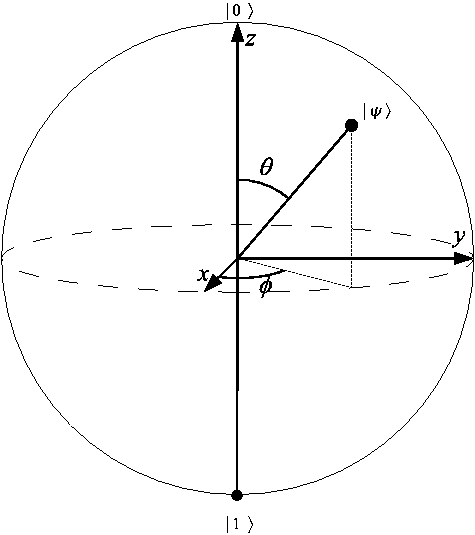
\includegraphics[scale=0.5]{Bloch.png}
\caption{The 1-Qubit Bloch Sphere \cite{QuantikiBlochSphereImage}}
\label{BlochSphere}
\end{figure}

%%REWORDED
A quantum state can be visualised as a point of the Bloch sphere, shown in Figure \ref{BlochSphere}, that represents the quantum state space.
The shown Bloch sphere is for a single qubit, the principle can be extended to $n$ qubits however the visualisation breaks down.
All quantum states can be described using the Bloch sphere.
The states that this project is concerned with are those that lie on the surface of the respective Bloch sphere, known as ``pure'' states.
%%

In quantum mechanics, a Ket is used to indicate a state, for example $\ket{0}$ is the state equivalent to logical $0$ whereas $\ket{1}$ is the state equivalent to logical $1$.

A dual to the Ket notation is the Bra notation, $\bra{a}$.
This notation is used to denote the ``dual vector'' of the corresponding Ket.
For a state vector represented by Equation \ref{ket_explanation_example} there is a dual vector representing its Hermitian Conjugate, Equation \ref{bra_explanation_example}.
The Hermitian Conjugate of a vector is the transpose of the vector after each entry is replaced by its complex conjugate.
\begin{equation}
\label{ket_explanation_example}
\ket{a} = 
\begin{pmatrix}
a_1\\
a_2\\
a_3\\
\vdots \\
a_n
\end{pmatrix}
\end{equation}
\begin{equation}
\label{bra_explanation_example}
\bra{a} = 
\begin{pmatrix}
a_1^{*}&
a_2^{*}&
a_3^{*}&
\cdots &
a_n^{*}
\end{pmatrix}
\end{equation}

Combining the two vectors $\bra{a}$ and $\ket{b}$, written $\bra{a}\ket{b}$, represents the inner product of the two vectors, $\ket{a}$ and $\ket{b}$.
If a and b are unit vectors and $a == b$, $\bra{a}\ket{b} == 1$.
If a and b are orthogonal, $\bra{a}\ket{b} == 0$.

The outer product of two vectors, $\ket{a}$ and $\ket{b}$, can be represented by $\ket{a}\bra{b}$.
This represents the transformation from $\ket{a}$ to $\ket{b}$.
It can also be represented in matrix form.

With
$\ket{0}
== 
\begin {pmatrix}
1\\
0\\
\end{pmatrix}
$
and
$\ket{1}
==  
\begin {pmatrix}
0\\
1\\
\end{pmatrix}
$
it is possible to represent single qubit operations in the ``Bra-Ket'' notation.
For example, the NOT gate performs a simple negation of a qubit's value.
This can be written as $\ket{0}\bra{1} + \ket{1}\bra{0}$.
Substituting in the vector values we have:
\begin{equation}
\begin{tabular}{ r c l }
\(\begin {pmatrix}
1\\
0
\end{pmatrix}
\begin {pmatrix}
0&&
1
\end{pmatrix}
 + 
\begin {pmatrix}
0\\
1
\end{pmatrix}
\begin {pmatrix}
1&&
0
\end{pmatrix}\)
& \(=\)
& \( 
\begin{pmatrix}
0 && 1 \\
0 && 0
\end{pmatrix}
 + 
\begin{pmatrix}
0 && 0\\
1 && 0
\end{pmatrix}
\) \\
& \(=\)
& \( 
\begin{pmatrix}
0 && 1 \\
1 && 0
\end{pmatrix}
\)
\end{tabular}
\label{eq:notexplanded}
\end{equation}

This matrix can be seen as a transformation matrix for the NOT operation.
In quantum computation, the NOT gate is one of the $4$ gates known as the Pauli gates, more specifically it is the Pauli-X gate.
It is called the Pauli-X gate as it can be seen as a rotation of $\pi$ radians about the X axis of the Bloch sphere, Figure \ref{BlochSphere}.
The Pauli gates are named after Wolfgang Pauli who published the matrices that define them.

% Definition of Unitary
The matrices representing the Pauli-X gate and all other quantum logic gates are \emph{unitary}.
A unitary matrix, U, is one which adheres to Equation \ref{eqn:unitarydef} where $I_n$ is the identity matrix in $n$ dimensions and $U^{\dagger}$ is the Hermitian Conjugate of $U$.
\begin{equation}
\label{eqn:unitarydef}
U^{\dagger}
U == UU^{\dagger} = I_n
\end{equation}

% Reversible logic
%%REWORDED
Unitary transformations are physically reversible.
Some classical gates are not.
For example, the AND operation looses information about the inputs and can be represented as the function $AND(a,b)\rightarrow{a\wedge{b}}$.
However, for practical purposes it is possible to produce physically reversible versions by incorporating supplementary information in the output.
For the AND operation both inputs have to be provided in the output so the function becomes $AND(a,b)\rightarrow{(a,b,a\wedge{b})}$.
%%

%Superposition
All the details of quantum computation introduced so far do not offer anything more than classical computation.
The power of quantum computation comes from the use of superposition.
Superposition is the ability of a qubit to be in both the $\ket{0}$ and $\ket{1}$ states simultaneously with certain probabilities.
It is not possible to observe the superposition of a qubit.
When observed the superposition ``collapses'' to either $\ket{0}$ or $\ket{1}$, the computational basis states.
The probability of the superposition collapsing to a specific state is determined by the superposition's complex amplitudes.

\begin{equation}
\label{superposition_explanaiton}
\alpha\vert0\rangle+\beta\vert1\rangle
\end{equation}

The notation for the superposition of states that a qubit is currently in is shown in Equation \ref{superposition_explanaiton}.
% It is the same as for the basis states except the values of $\alpha$ and $\beta$ are omitted when writing the basis states.
$\alpha$ and $\beta$ are the probability amplitudes for the respective states and are expressed as complex numbers.
The complex probability amplitudes have phases that can interfere with each other through computation.
However, only relative phase factors can be observed.
The probability of the state in Equation \ref{superposition_explanaiton} collapsing to the basis state $\ket{0}$ is given by $\vert\alpha\vert^2$.
Similarly, the probability of this state collapsing to the basis state $\ket{1}$ is $\vert\beta\vert^2$.
The overall probability of a superposition collapsing to any of the states it contains must equal $1$.
For the basis state $\ket{0}$ $\alpha==1$ and $\beta==0$ whereas for the basis state $\ket{1}$ $\alpha==0$ and $\beta==1$.
Any state where $\alpha$ and $\beta$ do not equal $1$ and $0$ is in superposition.

The state $\frac{1}{\sqrt{2}}\ket{0}+\frac{1}{\sqrt{2}}\ket{1}$ is an equal superposition where the collapse under observation to $\ket{0}$ is just as likely as collapsing to $\ket{1}$, probabilities of $|\frac{1}{\sqrt{2}}|^2=\frac{1}{2}$.
With $n$ qubits in equal superposition, there are $n$ binary values that have an equal probability of taking the value $0$ as the value $1$.
With an ordering decided of these qubits, collapsing the superposition of each qubit will result in a binary value of length n.
With the probabilities of each qubit being $\frac{1}{2}$ this binary value takes a truly random value between $0$ and $2^n-1$.
It is not possible to produce a truly random number using a classical computer.
Equation \ref{superposition_explanaiton_sum} is a generalisation for the equal superposition state over $n$ qubits.

\begin{equation}
\label{superposition_explanaiton_sum}
\frac{1}{\sqrt[n]{2}}\sum\limits_{i=0}^N \ket{x_i}
\end{equation}

In 1935, Erwin Schr$\ddot{o}$ginger\cite{SchroedingersCat} proposed a thought experiment to explain the idea of superposition.
Imagine a cat in a fully opaque box with a vial of poison.
The vial may break at any time, a truly random variable.
After sealing the box the liveness state of the cat is not known.
The cat could be alive if the vial has not broken but could just as likely be dead.
Only by looking inside the box will the state of the cat be known.
Until this time the cat could be thought of as both alive and dead at the same time.
If we assign ``dead'' to the state $\ket{0}$ and ``alive'' to the state $\ket{1}$ the situation looks very similar to the state in Equation \ref{superposition_explanaiton} where both both $\alpha$ and $\beta$ equal $\frac{1}{\sqrt{2}}$.
Therefore, just as the cat can be thought of as both dead and alive at the same time, a qubit in the superposition $\frac{1}{\sqrt{2}}\vert0\rangle+\frac{1}{\sqrt{2}}\vert1\rangle$ can be thought of both in the $\ket{0}$ and $\ket{1}$ states at the same time.
This leads to a very powerful property of quantum computers.
With $n$ classical bits, a single number in the range $0$ to $2^n-1$ can be expressed at any one time.
However with $n$ quantum qubits, every number in the range $0$ to $2^n-1$ can be expressed at the same time.

Quantum mechanics is said to be linear and unitary operations can distribute over linear sums.
As a quantum state can be expressed as the linear sum in Equation \ref{superposition_explanaiton_sum} the computation over all $2^n$ inputs to be performed in parallel.
This is represented by Equation\ref{eqn:uequiv}.%%%%%%%%%%%%%%%%%

\begin{equation}
\label{eqn:uequiv}
 U\sum_{x=0}^{2^n-1}\ket{x}\equiv{\sum_{x=0}^{2^n-1}U\ket{x}}
\end{equation}

This parallelism is very powerful and has been shown to enable the computation of problems classified as NP to be performed in polynomial time.
For example the factorisation algorithm discoved by Peter Shor\cite{Shor:1994jg}.
This does however have a caveat.
As mentioned previously the superposition cannot itself be observed.
When observation is attempted, the superposition collapses to a basis state with respect to the superposition probability amplitudes.
This means that even though $2^n$ calculations can be performed in parallel, only a single answer can be observed.

% mathematic examples of matrices and the application
Non-measurement operations that can be performed on quantum states are unitary and the Pauli-X operation is just one such operation.
Along with the Pauli-X gate, there are an additional 3 Pauli gates.
The Pauli-I gate is the simplest of all quantum gates.
It is the identity gate, the output is identical to the input.
In Dirac notation this is $\ket{0}\bra{0} + \ket{1}\bra{1}$, and Equation \ref{eqn:pauliicalc} shows the matrix form. 
\begin{equation}
\label{eqn:pauliicalc}
\begin{tabular}{ r c l }
\(\begin {pmatrix}
1\\
0
\end{pmatrix}
\begin {pmatrix}
1&&
0
\end{pmatrix}
 + 
\begin {pmatrix}
0\\
1
\end{pmatrix}
\begin {pmatrix}
0&&
1
\end{pmatrix}\)
& \(=\)
& \( 
\begin{pmatrix}
1 && 0 \\
0 && 0
\end{pmatrix}
 + 
\begin{pmatrix}
0 && 0\\
0 && 1
\end{pmatrix}
\) \\
& \(=\)
& \( 
\begin{pmatrix}
1 && 0 \\
0 && 1
\end{pmatrix}
\)
\end{tabular}
\end{equation}

The Pauli-Z gate rotates the quantum state by $\pi$ radians about the Z axis.
This represents a phase flip of the quantum state.
The phase of a state is important when interference is used in computation.
In Dirac notation this is $\ket{0}\bra{0} + \ket{1}(-\bra{1}$), and Equation \ref{eqn:paulizcalc} shows the matrix form.
\begin{equation}
\label{eqn:paulizcalc}
\begin{tabular}{ r c l }
\(\begin {pmatrix}
1\\
0
\end{pmatrix}
\begin {pmatrix}
1&&
0
\end{pmatrix}
 + 
\begin {pmatrix}
0\\
1
\end{pmatrix}
\begin {pmatrix}
0&&
-1
\end{pmatrix}\)
& \(=\)
& \( 
\begin{pmatrix}
1 && 0 \\
0 && 0
\end{pmatrix}
 + 
\begin{pmatrix}
0 && 0\\
0 && -1
\end{pmatrix}
\) \\
& \(=\)
& \( 
\begin{pmatrix}
1 && 0 \\
0 && -1
\end{pmatrix}
\)
\end{tabular}
\end{equation}

The Pauli-Y gate is similar to both the Pauli-X and Pauli-Z gates, but differs in the axis about which it performs the rotation.
The Pauli-Y gate rotates the quantum state by $\pi$ radians about the Y axis.
% This represents a phase flip followed by a bit flip.
In Dirac notation this is $\ket{0}(i\bra{1}) + \ket{1}(-i\bra{0}$), and Equation \ref{eqn:pauliycalc} shows the matrix form.
\begin{equation}
\label{eqn:pauliycalc}
\begin{tabular}{ r c l }
\(\begin {pmatrix}
1 \\
0
\end{pmatrix}
\begin {pmatrix}
0 &&
-i
\end{pmatrix}
 + 
\begin {pmatrix}
0 \\
1
\end{pmatrix}
\begin {pmatrix}
i &&
0
\end{pmatrix}\)
& \(=\)
& \( 
\begin{pmatrix}
0 && -i \\
0 && 0
\end{pmatrix}
 + 
\begin{pmatrix}
0 && 0\\
i && 0
\end{pmatrix}
\) \\
& \(=\)
& \( 
\begin{pmatrix}
0 && -i \\
i && 0
\end{pmatrix}
\)
\end{tabular}
\end{equation}

Along with the single qubit operations, like those above, there are operations which can act over $n$ qubits.
A simple example of a 2 qubit operation is the Controlled-NOT(CNOT) operator.
This is a simple extension of the Pauli-X gate.

\begin{table}
\centering
\begin{tabular}{ c | c || c | }
Control & Target Before & Target After \\
$\ket{0}$ & $\ket{0}$ & $\ket{0}$ \\
$\ket{0}$ & $\ket{1}$ & $\ket{1}$ \\
$\ket{1}$ & $\ket{0}$ & $\ket{1}$ \\
$\ket{1}$ & $\ket{1}$ & $\ket{0}$ \\
\end{tabular}
\caption{Classical CNOT Truth Table}
\label{CNOTTruthTable}
\end{table}

The CNOT gate has a control qubit which is required to be in the state $\ket{1}$ for the NOT operation on the target qubit to be carried out.
In classical logic this would extend the truth table to be as shown in Table \ref{CNOTTruthTable}.
The truth table of the CNOT gate is the same as that of the classical XOR gate.
The Dirac notation of the CNOT gate is $\ket{00}\bra{00}+\ket{01}\bra{01}+\ket{10}\bra{11}+\ket{11}\bra{10}$.

Circuit representations of the CNOT gate are shown in Figure \ref{fig:controlnotcir}.
Both the circuit representations are equivalent with the upper qubit as the control qubit with the lower qubit as the target.
The circuit in Figure \ref{fig:controlnotcirshort} shows the widely used shorthand for the CNOT gate with
$
 \Qcircuit @C=1.0em @R=.7em {
& \targ & \qw& \\
}
$
representing the Pauli-X operation.

\begin{figure}
\centering
 \subfigure[]{
$
 \Qcircuit @C=1.0em @R=.7em {
& \ctrl{1} & \qw & \\
& \gate{X} & \qw& \\
& & &
}
$
}
\hspace{20pt}
 \subfigure[]{
$
 \Qcircuit @C=1.0em @R=.7em {
& \ctrl{1} & \qw & \\
& \targ & \qw& \\
& & &
}
$
\label{fig:controlnotcirshort}
}
\caption{Controlled Not Gate}
\label{fig:controlnotcir}
\end{figure}


\begin{figure}
\centering
\subfigure[Basic Circuit]{\label{fig:singatetwocirsubfig1}
$
 \Qcircuit @C=1.0em @R=.7em {
&&&&& \gate{X}& \qw &&&& \\
&&&&& \qw& \qw&&&& \\
&&&&& & &&&&
}
$
}
\subfigure[Full Circuit]{\label{fig:singatetwocirsubfig2}
$
\Qcircuit @C=1.0em @R=.7em {
&&&&& \gate{X} & \qw&&&&\\
&&&&& \gate{I}& \qw&&&&\\
&&&&& & &&&&
}
$
}
\subfigure[Corresponding Circuit]{\label{fig:singatetwocirsubfig3}
$
\Qcircuit @C=1.0em @R=.7em {
&&&&& \multigate{1}{\mathcal{F}} & \qw&&&&\\
&&&&& \ghost{\mathcal{F}}& \qw&&&&\\
&&&&& & &&&&
}
$
}
\caption{Single Qubit Gate, 2 Qubit Circuit}
 \label{fig:singatetwocir}
\end{figure}

For a $2$ qubit circuit, the state has $4$ elements in the state vector.
This means that to apply a single qubit gate to this state, multiply the state by the respective $2\times{2}$ unitary matrix, there will be a problem due to the matrix dimensions not matching.
The matrix of the single qubit gate has to be expanded to a $4\times{4}$ matrix so that it can be applied to the state vector.
Taking the circuit shown in Figure \ref{fig:singatetwocirsubfig1} as an example we can see that the it is a simple Pauli-X gate, bit-flip operator, acting on the higher order qubit while nothing occurs to the lower order qubit.
Nothing happening to the lower order qubit is the same as applying the Pauli-I gate, identity operator, to this qubit.
The circuit in Figure \ref{fig:singatetwocirsubfig2} shows the resulting circuit with identical effect on all possible input states.
This interpretation of the circuit still doesn't provide a solution as there are separate $2\times{2}$ matrices for each of the two gates.
These can't be applied to the state individually for that same reason as before.

To produce a $4\times{4}$ matrix for the circuit, the two $2\times{2}$ matrices have to be combined.
The matrix operation that is used for this is the Tensor Product.
The tensor product is a simple matrix operation that is denoted using the $\otimes$ symbol.
The result of the tensor product operation is shown in Equation \ref{eq:tensorop}.

\begin{eqnarray}
A \otimes B = 
\begin{pmatrix}
a_{00} && a_{01} \\
a_{10} && a_{11}
\end{pmatrix}
\otimes
\begin{pmatrix}
b_{00} && b_{01} \\
b_{10} && b_{11}
\end{pmatrix}
&=&
\begin{pmatrix}
a_{00}B && a_{01}B \\
a_{10}B && a_{11}B
\end{pmatrix} \nonumber \\
&=&
\begin{pmatrix}
a_{00}b_{00} && a_{00}b_{01} & a_{01}b_{00} && a_{01}b_{01}\\
a_{00}b_{10} && a_{00}b_{11} & a_{01}b_{10} && a_{01}b_{11}\\
a_{10}b_{00} && a_{10}b_{01} & a_{11}b_{00} && a_{11}b_{01}\\
a_{10}b_{10} && a_{10}b_{11} & a_{11}b_{10} && a_{11}b_{11}
\end{pmatrix}
\label{eq:tensorop}
\end{eqnarray}

So when applying this to the matrices of Pauli-X as A and the Pauli-I as B we get the unitary matrix for the corresponding $\mathcal{F}$ gate, shown in Figure \ref{fig:singatetwocirsubfig3}.
This can be seen in Equation \ref{eq:tensoropXI}.

\begin{eqnarray}
  \mathcal{F} =
X \otimes I =
\begin{pmatrix}
0 && 1\\
1 && 0
\end{pmatrix}
\otimes
\begin{pmatrix}
1 && 0 \\
0 && 1
\end{pmatrix} & = & \begin{pmatrix}
0I && 1I \\
1I && 0I
\end{pmatrix}  \nonumber \\
   & = & \begin{pmatrix}
0\times{1} && 0\times{0} & 1\times{1} && 1\times{0}\\
0\times{0} && 0\times{1} & 1\times{0} && 1\times{1}\\
1\times{1} && 1\times{0} & 0\times{1} && 0\times{0}\\
1\times{0} && 1\times{1} & 0\times{0} && 0\times{1}
\end{pmatrix} \nonumber  \\
   & = & \begin{pmatrix}
0 && 0 & 1 && 0\\
0 && 0 & 0 && 1\\
1 && 0 & 0 && 0\\
0 && 1 & 0 && 0
\end{pmatrix}
\label{eq:tensoropXI}
\end{eqnarray}

Tensor product scales to any number of qubits and can therefore produce $2^n\times{2^n}$ matrices for systems involving $n$ qubits.
The tensor product cannot however be used in this same way to produce unitary matrices for controlled gates.
It can only be used when the action on each qubit is independent.

More than two matrices be combined by the tensor product operation, $A\otimes{B}\otimes{C}$.
The operation is broken down from right to left into a number of two qubit operations, $A\otimes(B\otimes{C})$.
The ordering of the matrices is important.
Assuming $A$, $B$ and $C$ are single qubit quantum operations the operation encoded by $A$ would operate on the highest significant qubit while the operation encoded by $C$ would operate on the lowest significant qubit.
The operation encoded by $B$ would operate on the middle qubit.

%Entanglement

Not all multiple qubit states can be expressed as the tensor products of individual states.
Such states are said to be entangled.
An example with two qubits is the state $\frac{1}{\sqrt{2}}(\ket{00}+\ket{11})$.
This state cannot be factored into two quantum states, one for each qubit.
This is also a superposition of two states and under observation the superposition will collapse to one of $\ket{00}$ or $\ket{11}$.
Thus when one of the qubits is observed and is seen to be in state $\ket{0}$ we can deduce that that the other qubit is also in the state $\ket{0}$.
Similarly, if the qubits were observed to be in the state $\ket{1}$ we can deduce that that the other qubit is also in the state $\ket{1}$.
% What is important to not is that if we are to observe one of the qubits in this state, it is possible to know the state of the other qubit without observing it.
% Taking the example state, if the higher significant qubit is observed to be in the state $\ket{0}$ it can be deduced that the lower significant qubit is also in the state $\ket{0}$ 
% The same is true if the higher significant qubit is observed to be in the state $\ket{1}$, the lower significant qubit is also in the state $\ket{1}$
It is important to note that this property is maintained regardless of spacial separation.


\section{An Introduction to Quantum Circuits and Algorithms}
%Known Quantum Algorithms

Quantum computational artefacts can be considered at various levels of abstraction.
At the implementation level computation is the application of a sequence of specific operations.
This sequence of operations shall be referred to as a circuit.
A circuit generally operates over a quantum system of a fixed size, referred to as the system size.
For example a circuit could invert, by applying the Pauli-X operation, each qubit of a three qubit state.
A program is an artefact that when evaluated produces a circuit.
An algorithm is an artefact that when instantiated with the system size produces a program.
This relationship can be seen in Figure \ref{fig:comartefacts}.

\begin{figure}[ttt!]
\centering
\begin{minipage}[b]{0.2\textwidth}
\begin{tabular}{c}
\textbf{Circuit Artefact}
\\
$
\Qcircuit @C=1.0em @R=.7em {
&&& \\
&\gate{X} &\qw&\\
&\gate{X} &\qw&\\
&\gate{X} &\qw& \\
&&& \\
&&&
}
$
\end{tabular}
\end{minipage}
\hfill
\begin{minipage}[b]{0.3\textwidth}
\begin{algorithm}[H]
\caption{Program Artefact} 
\label{alg1} 
\begin{algorithmic}
\FOR{$i : 1 \rightarrow 3 : i++$}
 \STATE $Pauli-X(i)$
\ENDFOR
\end{algorithmic}
\end{algorithm}
\end{minipage}
\hfill
\begin{minipage}[b]{0.4\textwidth}
\begin{algorithm}[H]
\caption{Algorithm Artefact} 
\label{alg2} 
 \begin{algorithmic}
 \FOR{$i : 1 \rightarrow System\_Size : i++$}
 \STATE $Pauli-X(i)$
\ENDFOR
\end{algorithmic}
\end{algorithm}
\end{minipage}
\hfill
\caption{Computational Artefacts}
\label{fig:comartefacts}
\end{figure}

% Just as with classical computation, the circuit used to perform computation can be designed in several ways.
% Classical circuits can be designed directly as a sequence of logic gates.
% The processing can also be designed at a slightly higher level using an algorithm.
% Algorithms are ordered lists of instructions that can include control flow constructs such as loops.
% Algorithms can include variables such as the number of qubits in the system and the loop counters.
% With the number of qubits defined the algorithm can be instantiated to produce a program.
% 
% An instantiated algorithm, with the parameters set to certain values, is referred to as a program.
% Design can also directly produce these programs if the parameters are fixed before the design process.

This gives three artefacts, each at a different level of abstraction that can be designed to specify a solution to a problem.
\begin{itemize}
 \item A circuit
 \item A program
 \item An algorithm
\end{itemize}

The same is true for quantum artefact design.
The design can either be done at the circuit level, program level or parametrisable algorithm level.

Currently there are very few problems for which a quantum solution is known.
Peter Shor published a discussion on the progress made ``in discovering algorithms for computation on a quantum computer''\cite{Shor:2004:PQA:1032132.1032149}.
Shor suggests two possible reasons for the lack of quantum algorithms.
The first was ``that there might really be only a few problems for which quantum computers can offer a substantial speed-up over classical computers''\cite{Shor:2004:PQA:1032132.1032149}.
This would indeed make the discovery of useful quantum algorithms difficult.
However, I feel this is rather pessimistic.
The main focus of the paper published by Feynman\cite{Feynman82simulatingphysics} was the problem of simulating the physics of quantum mechanics on a classical computer.
This suggests there the potential of many applications for quantum computers, even if they aren't analogous to classical computational applications.

The second reason was ``that quantum computers operate in a manner so non-intuitive, and so different from classical computers''\cite{Shor:2004:PQA:1032132.1032149} that our current algorithm knowledge is close to useless.
This, in my opinion, is a much more significant obstacle.
Quantum mechanics is seen by many as a confusing and mystical subject.
Prize winning mathematician and physicist Roger Penrose is attributed to the remark ``Quantum mechanics makes absolutely no sense''.
Statements such as this do nothing to promote the universal study of quantum mechanics.
If quantum mechanics and other subjects, such as general relativity, were, even in part, to filter into curricula I feel general understanding would improve, leading to greater intuition.
Without this it may simply be unreasonable to expect discoveries that exploit the finer details of these complex and subtle theories to become frequent occurrences.
I think this applies to many areas of research including quantum computation.

Research into the use of heuristic search techniques to assist in the design of quantum algorithms has shown promise.
Several different techniques have been used to varying success.
Not only do the techniques differ, but so do the target artefacts.
Research has been presented to design at each of the three levels of abstraction outlined above.

In the following sections several quantum algorithms shall be explained in detail.
This is followed by an overview of the research that has been carried out using heuristic search to perform quantum algorithm synthesis.

\subsection{Deutsch Algorithms}
\label{sec:DeutAlg}
In 1985, Deutsch\cite{Deutsch85quantumtheory} proposed a probabilistic solution to a simple promise problem.
The solution was improved to a deterministic solution by Cleve et al.\cite{Cleve98quantumalgorithms}.
Despite the improvement being produced by Cleve et al. the algorithm is popularly known as the Deutsch algorithm.
% The algorithm presented in \cite{Deutsch85quantumtheory} was the first application where quantum computation was shown to be provably faster than classical computation.

The Deutsch algorithm is intended to solve the following problem:
\begin{quote}
Given a function $f:\{0,1\}\to\{0,1\}$, state whether it is either a balanced, or constant function.
The ``promise'' is that the function $f$ is guaranteed to be either balanced or constant.
\end{quote}
The algorithm's major breakthrough was that it only required a single invocation of the function $f$ to decide in which category it belonged.
The best classical approach requires two invocations.
This was the first algorithm to exploit quantum mechanics to compute the solution to a problem provably more efficiently, with efficiency defined as the number of evaluations of $f$, than a classical solution.

\begin{figure}
\[
\Qcircuit @C=1.0em @R=.7em {
&			&  1 &		&  2 &				&  3 &		&  4 &		\\
& \lstick{\ket{0}} 	& \qw& \gate{H} & \qw& \gate{f} 	& \qw& \gate{H} &\qw& \meter \\
& \lstick{\ket{1}} 	& \qw& \gate{H} & \qw& \targ\qwx 		& \qw& \qw	&\qw& \rstick{\ket{0}-\ket{1}}\qw  
}
\]
\caption{Deutsch Circuit}
 \label{Deutsch-Cir}
\end{figure}

The circuit for this algorithm is presented in Figure \ref{Deutsch-Cir}.
Despite this being known as the Deutsch Algorithm, the solution is a circuit rather than a parametrisable list of instruction.
The mathematical reasoning does not scale to functions with greater than a single input qubit.
Between points $2$ and $3$ in Figure \ref{Deutsch-Cir} is a modified Controlled-Not gate.
The standard Controlled-Not gate uses the value of the control qubit to decide whether to perform the Pauli-X operation.
This modified gate does not use the control qubit value, $x$, but the result of the $f(x)$ to decide whether to perform the Pauli-X operation.
However, just as with the standard Controlled-Not gate, this modified version does not affect the value of the qubits used by the control function.

% Before the maths of the algorithm can be introduced, a few equivalences and definitions need to be introduced.
% These are formally stated in Equations \ref{target_qubit_identity} to \ref{eqn:deutschevalgen}.
% 
% \begin{equation}
% \ket{a}(\ket{c}-\ket{b})\equiv\ket{a}(-1(\ket{b}-\ket{c}))\equiv-1\ket{a}(\ket{b}-\ket{c})
% \label{target_qubit_identity}
% \end{equation}
% \begin{equation}
% \label{eqn:deutschevalzero}
%  \ket{x}\frac{1}{\sqrt{2}}(\ket{0}-\ket{1}) \xrightarrow{f} \ket{x}\frac{1}{\sqrt{2}}(\ket{0}-\ket{1})
% \end{equation}
% \begin{equation}
% \label{eqn:deutschevalone}
%  \ket{x}\frac{1}{\sqrt{2}}(\ket{0}-\ket{1}) \xrightarrow{f} -\ket{x}\frac{1}{\sqrt{2}}(\ket{0}-\ket{1})
% \end{equation}
% \begin{equation}
% \label{eqn:deutschevalgen}
%  \ket{x}\frac{1}{\sqrt{2}}(\ket{0}-\ket{1}) \xrightarrow{f} (-1)^{f(x)}\ket{x}\frac{1}{\sqrt{2}}(\ket{0}-\ket{1})
% \end{equation}
% 
% \begin{list}{}{\topsep=0cm,\itemsep=0cm}
%   \item Equation \ref{target_qubit_identity} is used to simplify Equations \ref{eqn:deutschevalzero} and \ref{eqn:deutschevalone} so the state of the second qubit remains as $\frac{1}{\sqrt{2}}(\ket{0}-\ket{1})$.
%   \item Equation \ref{eqn:deutschevalzero} is the effect $f$ has on state $\ket{x}\frac{1}{\sqrt{2}}(\ket{0}-\ket{1})$ when $f(x)=0$.
%   \item Equation \ref{eqn:deutschevalone} is the effect $f$ has on state $\ket{x}\frac{1}{\sqrt{2}}(\ket{0}-\ket{1})$ when $f(x)=1$.
%   \item Equation \ref{eqn:deutschevalgen} is the combination of Equations \ref{eqn:deutschevalzero} and \ref{eqn:deutschevalone} to produce the generalised equation for the effect $f$ has on state $\ket{x}\frac{1}{\sqrt{2}}(\ket{0}-\ket{1})$.
% \end{list}
% 
% Equations \ref{eqn:deutschstart} to \ref{Deutsch_final_state} provide full details of the maths behind the way the circuit in Figure \ref{Deutsch-Cir} produces its result.
% 
% \begin{equation}
% \label{eqn:deutschstart}
% \ket{01} \xrightarrow{H\otimes{H}} \frac{1}{\sqrt{2}}(\ket{0}+\ket{1})\frac{1}{\sqrt{2}}(\ket{0}-\ket{1})
% \end{equation}
% \begin{equation}
% \label{eqn:deutschevalsuper1}
%  \frac{1}{\sqrt{2}}(\ket{0}+\ket{1})\frac{1}{\sqrt{2}}(\ket{0}-\ket{1}) \xrightarrow{f} \frac{1}{\sqrt{2}}((-1)^{f(0)}\ket{0}+(-1)^{f(1)}\ket{1})\frac{1}{\sqrt{2}}(\ket{0}-\ket{1})
% \end{equation}
% \begin{equation}
% \label{eqn:deutschevalsuper2}
%  \frac{1}{\sqrt{2}}((-1)^{f(0)}\ket{0}+(-1)^{f(1)}\ket{1})\frac{1}{\sqrt{2}}(\ket{0}-\ket{1}) \equiv (-1)^{f(0)}\frac{1}{\sqrt{2}}(\ket{0}+(-1)^{f(0)\oplus{f(1)}}\ket{1})\frac{1}{\sqrt{2}}(\ket{0}-\ket{1})
% \end{equation}
% \begin{equation}
%  \frac{1}{\sqrt{2}}(\ket{0}+(-1)^{f(0)\oplus{f(1)}}\ket{1})
% \label{Deutsch_final_state}
% \end{equation}
% 
% \begin{list}{}{\topsep=0cm,\itemsep=0cm}
%   \item Equation \ref{eqn:deutschstart} is the transition between the points labelled $1$ and $2$ in Figure \ref{Deutsch-Cir}.
%   \item Equation \ref{eqn:deutschevalsuper1} is the transition between the points labelled $2$ and $3$ in Figure \ref{Deutsch-Cir}. This is simplified using the generalisation made in Equation \ref{eqn:deutschevalgen}.
%   \item Equation \ref{eqn:deutschevalsuper2} is the some algebraic manipulation of Equation \ref{eqn:deutschevalsuper1}.
%   \item Equation \ref{Deutsch_final_state} is the simplification of Equation \ref{eqn:deutschevalsuper2}.
% As only the higher significant qubit is ever observed and the global phase factor $(-1)^{f(0)}$ cannot be observed, neither affect the observation so can be omitted from the equation.
% This simplification is made easier by all the previous steps being simplified with Equation \ref{target_qubit_identity} where possible as the state of the lower significant qubit is the same as at the point labelled $1$ in Figure \ref{Deutsch-Cir}.
% \end{list}
% 
% \begin{equation}
%  \frac{1}{\sqrt{2}}(\ket{0}+(-1)^{f(0)\oplus{f(1)}}\ket{1}) \equiv \frac{1}{\sqrt{2}}(\ket{0}-\ket{1})
% \label{eqn:deutschpoint3bal}
% \end{equation}
% \begin{equation}
%  \frac{1}{\sqrt{2}}(\ket{0}-\ket{1}) \xrightarrow{H} \ket{1}
% \label{eqn:deutschpoint4bal}
% \end{equation}
% \begin{equation}
%  \frac{1}{\sqrt{2}}(\ket{0}+(-1)^{f(0)\oplus{f(1)}}\ket{1}) \equiv \frac{1}{\sqrt{2}}(\ket{0}+\ket{1})
% \label{eqn:deutschpoint3const}
% \end{equation}
% \begin{equation}
%  \frac{1}{\sqrt{2}}(\ket{0}+\ket{1}) \xrightarrow{H} \ket{0}
% \label{eqn:deutschpoint4const}
% \end{equation}
% 
% When f is balanced the state at the point labelled $3$ in Figure \ref{Deutsch-Cir} is Equation \ref{eqn:deutschpoint3bal} as $f(0) \oplus f(1) = 1$ due to either $f(0)$ or $f(1)$ evaluating to $1$ but not both.
% When this is passed through the final Hadamard it produces Equation \ref{eqn:deutschpoint4bal}.
% 
% When f is constant the state at the point labelled $3$ in Figure \ref{Deutsch-Cir} is Equation \ref{eqn:deutschpoint3const} as $f(0) \oplus f(1) = 0$ due to $f(0)$ and $f(1)$ both evaluating to $0$ or both evaluating to $1$.
% However, when this is passed through the final Hadamard it produces Equation \ref{eqn:deutschpoint4const}.
% This means that using just a single query to the function $f(x)$, the algorithm can provide an answer to the problem.

However in the circuit shown in Figure \ref{Deutsch-Cir}, when the modified Controlled-Not operation is activated by $f(\ket{0})$ it can be seen as a phase flip on the state $\ket{0}$.
The same is true for the state $\ket{1}$.
This doesn't seem to follow either the operation previously given for the Pauli-X gate or the statement just made that the control qubit is not affected.
However, as the state of the lower qubit at label $2$ is $\frac{1}{\sqrt{2}}(\ket{0}-\ket{1})$ when the Pauli-X operation is applied the state is transformed to $\frac{1}{\sqrt{2}}(\ket{1}-\ket{0})$ which can be rewritten as $\frac{-1}{\sqrt{2}}(\ket{0}-\ket{1})$.
The negative sign propagates through the maths and can be viewed as acting on the upper qubit.

If the function is balanced only one of the two states of the upper qubit in the superposition will activate the Pauli-X operation.
This results in the effective phase flip applying on only one of the states inside the superposition
The resulting upper qubit state is equivalent to $\frac{1}{\sqrt{2}}(\ket{0}-\ket{1})$ regardless of whether $\ket{0}$ or $\ket{1}$ activates the Pauli-X operation as $-1$ can be factored out as unobservable global phase.
When the final Hadamard gate is applied to the state $\frac{1}{\sqrt{2}}(\ket{0}-\ket{1})$ the state of the upper qubit is $\ket{1}$.

If the function is constant both or neither of the states in the superposition, $\ket{0}$ and $\ket{1}$, activate Pauli-X operation.
If both activate the operation, the effective phase flip is applied to both the states inside the superposition resulting in a global, and therefore unobservable, phase flip.
This results in the upper qubit being in state $\frac{-1}{\sqrt{2}}(\ket{0}+\ket{1})$.
If neither activate the operation the upper qubit remains in the state $\frac{1}{\sqrt{2}}(\ket{0}-\ket{1})$.
The application of the final Hadamard gate on these states produces on the upper qubit the state $\pm\ket{0}$, with only $\ket{0}$ observable.

These two results are distinct.
A balanced function results in $\ket{1}$ and a constant function results in $\ket{0}$.

This algorithm is very neat and simple.
It performs in a deterministic manner and outperforms the classical equivalent.
It does however reinforce the statement made by Shor\cite{Shor:2004:PQA:1032132.1032149} regarding the lack of background knowledge that can be drawn upon to create these algorithms.
The construction of such an algorithm cannot be produced simply by understanding the concepts of classical algorithm design.

The main observation that should be taken from this algorithm is how the output is observed on the quibit that is not physically acted on by the modified CNOT gate.
As mentioned above, if the circuit between points $3$ and $4$ in Figure \ref{Deutsch-Cir} were analysed by hand as a classical circuit, the input qubit would not be affected.
However, when it becomes a quantum circuit with the addition of phase, the control qubit is affected.
This is a prime example where the solution requires the understanding of the subtle implications of complex probability amplitudes in superposition and the vision to exploit it.

\subsection{Deutsch-Jozsa Algorithm}
\label{sec:DeutJozsaAlg}

%Deutsch-Jozsa Algorithm
The Deutsch-Jozsa algorithm\cite{1992-deutsch} is a generalisation and improvement over the earlier Deutsch algorithm\cite{Deutsch85quantumtheory}.
The algorithm was improved by Cleve et al.\cite{Cleve98quantumalgorithms}.
The improved algorithm is still generally referred to as the Deutsch-Jozsa algorithm.

In 1992 David Deutsch and Richard Jozsa\cite{1992-deutsch} presented an extension to the Deutsch algorithm, Section \ref{sec:DeutAlg}, that allowed for functions $f:\{0,1\}^{2^n}\to\{0,1\}$ to be categorised as constant or balanced.
The algorithm was probabilistic and required 2 invocations to the function $f$.
This means that in the worst case, with $n=1$, the algorithm will perform worse than both the original Deutsch algorithm\cite{Deutsch85quantumtheory} and the classical algorithm due to the probabilistic nature of its result.
This is a very limited case and performance improves as the value of $n$ increases.
The improvement by Cleve et al. reduces this to a single invocation of the function $f$ and is deterministic.
As with the original Deutsch algorithm, the number of invocations of $f$ is constant, truly independent of both $n$ and $f$.
This is again an improvement over the classical algorithm which requires in the worst case $2^{n-1}+1$ to be certain of the function's classification.

\begin{figure}
\[
\Qcircuit @C=1.0em @R=.7em {
& \lstick{\ket{0}} & \gate{H} & \multigate{3}{\mathcal{F}} & \gate{H} & \meter \\
& \lstick{\ket{0}} & \gate{H} & \ghost{\mathcal{F}} & \gate{H} & \meter \\
& \lstick{\ket{0}} & \gate{H} & \ghost{\mathcal{F}} & \gate{H} & \meter \\
& \lstick{\ket{0}} & \gate{H} & \ghost{\mathcal{F}}  & \gate{H} & \meter \\
& \lstick{\ket{1}} & \gate{H} & \targ\qwx & \rstick{\ket{0}-\ket{1}}\qw   
}
\]
\caption{Deutsch-Jozsa Circuit}
 \label{Deutsch-Jozsa-Cir}
\end{figure}

The circuit that is produced by this algorithm is shown in Figure \ref{Deutsch-Jozsa-Cir}.
The algorithm requires $n$ input qubits and a single ancillary qubit.

% The $n$ input qubits are initialised to $\ket{0}$.
% The ancillary qubit is initialised to $\ket{1}$.
% The $n$ Hadamard gates are used to produce the superposition of all $0..2^n-1$ possible inputs, $x=(\ket{0}+\ket{1})^n$.
% The Hadamard gate on the control qubit is used to produce the superposition $\ket{0}-\ket{1}$.
% The difference in superposition between the input and control qubits is important to the way in which the algorithm classifies a function.
% This produces a state $\frac{1}{\sqrt{2^n}}(\ket{0}+\ket{1})^n\frac{1}{\sqrt{2}}(\ket{0}-\ket{1})$.
% 
% 
% % The n input qubits, in the superposition $(\ket{0}+\ket{1})^n$, are then passed to the function we wish to classify, $f(x)$.
% The result of $f(x)$ is used as the control for a CNOT gate acting on the ancillary qubit.
% Note at this point that the input $x$ is in effect all possible inputs to $f(x)$, and as such the output is all the respective outputs.
% This means that each of the elements of the input state are transformed, based on the action of $f(x)$.
% This can be formalised as $CNOT_{\mathcal{F}}(\ket{x},\ket{y})=(\ket{x},\ket{f(x)\oplus{y}})$.
% Using the final Hadamard gates we can use the transformation to categorise $f(x)$.
% 
% With $n=2$, after the initial Hadamard gates we have the superposition in Equation \ref{eqn:deutschJozsaStart}.
% \begin{equation}
% \frac{1}{2}\ket{\Psi_{init}}\frac{1}{\sqrt{2}}(\ket{0}-\ket{1})=\frac{1}{2}(\ket{00}+\ket{01}+\ket{10}+\ket{11})\frac{1}{\sqrt{2}}(\ket{0}-\ket{1})
% \label{eqn:deutschJozsaStart}
% \end{equation}
% The NOT operation on the ancillary qubit is only activated if $f(x)=1$ which, using the equivalence in Equation \ref{target_qubit_identity} also used in the the original Deutsch algorithm, produces the superposition $-1\ket{x}(\ket{0}-\ket{1})$.
% This can also be generalised as $(-1)^{f(x)}\ket{x}(\ket{0}-\ket{1})$ where $-1^1=-1$ and $-1^0=1$ by definition.
% \begin{equation}
% \frac{1}{2}((-1)^{f(00)}\ket{00}+(-1)^{f(01)}\ket{01}+(-1)^{f(10)}\ket{10}+(-1)^{f(11)}\ket{11})\frac{1}{\sqrt{2}}(\ket{0}-\ket{1})
% \label{eqn:deutschJozsaFin}
% \end{equation}
% 
% By linearity the superposition after the NOT controlled by $f(x)$ on the ancillary qubit is Equation \ref{eqn:deutschJozsaFin}.
% After the application of $f(x)$, the ancillary bit has served it purpose and is neither measured nor entangled with any of the qubits of the $n$ input qubits.
% To simplify the equations the $(\frac{1}{\sqrt{2}}\ket{0}-\ket{1})$ contributed by the target qubit is ignored, the remaining state will be refereed to as $\Psi$.
% \begin{equation}
% \label{eqn:psiconst}
% \ket{\Psi_{const}}=\pm\frac{1}{2}(\ket{00}+\ket{01}+\ket{10}+\ket{11})
% \end{equation}
% \begin{equation}
% \label{eqn:psibal}
% \ket{\Psi_{bal}}=(-1)^{f(00)}\ket{00}+(-1)^{f(01)}\ket{01}+(-1)^{f(10)}\ket{10}+(-1)^{f(11)}\ket{11}
% \end{equation}
% If the function $f(x)$ is constant the state is Equation \ref{eqn:psiconst}.
% Whereas if $f(x)$ is balanced the state is Equation \ref{eqn:psibal}.
% However,as $\ket{\Psi_{const}}$ and $\ket{\Psi_{bal}}$ are orthogonal, Equation \ref{eqn:balconstorth}, it is possible to detect if the function is balanced or constant.
% \begin{equation}
% \label{eqn:balconstorth}
% \bra{\Psi_{bal}}\ket{\Psi_{const}}=0
% \end{equation}
% 
% Applying the $n$ Hadamard gates to the state $\Psi_{const}$ produces the state $\pm\ket{0}^{\otimes{n}}$.
% When measured this will return the result $\ket{0}^{\otimes{n}}$ as the global phase factor $\pm$ cannot be observed.
% With $\Psi_{const}$ and $\Psi_{bal}$ being orthogonal, the application of the $n$ Hadamard gates, which preserve orthogonality, to $\Psi_{bal}$ would result in an observation orthogonal to $\ket{0}^{\otimes{n}}$, i.e. any state other than $\ket{0}^{\otimes{n}}$.
% This gives a clear deterministic distinction between when $f$ is constant or balanced requiring just a single invocation of $f$.
% If the observation is $\ket{0}^{\otimes{n}}$ then $f(x)$ is constant, if the observation is any other state $f(x)$ is balanced.

The algorithm effectively works in the same way.
The only difference is that the state produced by each balanced function is potentially different.
% All that can be said for certain is that only a constant function can produce the observed state $\ket{0}^{\otimes{n}}$.
% As it is promised that the function is either constant or balanced this results in two distinct cases.
If the observed state is $\ket{0}^{\otimes{n}}$ the function $f$ is constant.
If the observed state is any other state the function $f$ is balanced.

The similarities between the original Deutsch algorithm and the more general Deutsch-Jozsa algorthim are quite apparent.
The Deutsch-Jozsa algorithm again uses superposition $\ket{0}-\ket{1}$ to cause an affect on the state of the input qubit when the action is physically performed on the ancillary qubit.

\subsection{Grover's Search Algorithm}	
\label{sec:grovers}
%Grovers Database search algorithm
The Grover Search algorithm\cite{Grover:1996rk} is a search problem to find a solution $x$ such that $f(x)=True$ for some predicate $f$.
The algorithm does not exploit or assume any structure, such as sorting, in the data set over which it is searching.

It has previously been proven\cite{Bennett:1996iu} that the lower complexity limit for any algorithm identifying an element without knowledge of underlying structure in the data is $\Omega(\sqrt{N})$.
$N$ represents the number of elements in the search space.
It is assumed $N=2^n$.
The complexity is measured by the number of elements which need to be queried in order to find the desired element.
The Grover Search algorithm has the complexity $O(\sqrt{N})$ and so ``is within a constant factor of the fastest possible quantum mechanical algorithm''\cite{Grover:1996rk}.

\begin{figure}
\begin{center}

\subfigure[Initialisation Circuit]{
\label{fig:groversinit}
$
\Qcircuit @C=1.0em @R=1.13em {
\ket{0}&&\qw&\qw &  \gate{H}  		&\qw 	&\qw&\qw\\
      &&\qw&\qw &  \vdots 		& 	&\qw&\qw\\
      &&\qw&\qw &  \vdots 		& 	&\qw&\qw\\
\ket{0}&&\qw&\qw &  \gate{H} 		&\qw 	&\qw&\qw\\
\ket{1}&&\qw&\qw &  \gate{H} 		&\qw	&\qw&\qw 
}
$
}
\hspace{20pt}
\subfigure[Repeated Circuit]{
 \label{Grovers-Search-Cir}
$
\Qcircuit @C=1.0em @R=.7em {
& \qw 		& \qw 	& \multigate{3}{f} 	&\qw 	&  \gate{H} 	&\qw 	& \multigate{3}{f_0} 	&\qw &  \gate{H}  	&\qw 	&\qw\\
& \vdots 	& 	&  \ghost{f} 		& \qw 	& \vdots 	& 	& \ghost{f_0} 		&\qw &  \vdots 		& 	&\qw\\
& \vdots 	& 	& \ghost{f} 		& \qw 	& \vdots 	& 	& \ghost{f_0} 		&\qw &  \vdots 		& 	&\qw\\
& \qw 		&\qw 	&  \ghost{f} 		& \qw 	& \gate{H} 	&\qw 	& \ghost{f_0} 		&\qw &  \gate{H} 	&\qw 	&\qw\\
& \qw 		&\qw 	&  \targ \qwx 		&\qw 	&  \qw 		&\qw 	& \targ \qwx 		&\qw &  \gate{X} 	&\qw	&\qw 
}
$}
 
\end{center}
\caption{Grover's Search Algorithm}
\end{figure}


The algorithm works for one or more solutions.
The number of solutions shall be represented by $M$.
Any state whose observation will provide one of the $M$ solutions solves the search problem.

The mechanisms used within the algorithm to produce a solution to the problem are more subtle than those used but the Deutsch-Jozsa algorithm.
The algorithm does not perform the computation in a single step.
After the initialisation circuit has been applied, see Firgure \ref{fig:groversinit}, the circuit shown in Figure \ref{Grovers-Search-Cir} is repeated in $O(\sqrt{N})$ times.
The actual number of times depends on $N$ and the number of solutions, $M$.

The algorithm works on amplification.
Each time the circuit is applied the probability amplitude of the desired solution is increased.

The application of Figure \ref{Grovers-Search-Cir} can be seen as rotating by $\sqrt{\frac{M}{N}}$ Radians around the Bloch Sphere of the $n$ qubit system, see Figure \ref{BlochSphere}.
The state $\ket{1}$ would represent the state in which only solutions have non-zero probability amplitudes.
The state $\ket{1}$ would represent the state in which only solutions have zero probability amplitudes.
After $\frac{\pi\sqrt{N}}{4\sqrt{M}}$ repetitions the probability of observing the correct state is the same as the combined probabilities of all other states after the circuit in Figure \ref{fig:groversinit} was initially applied.
The value of $M$ is required to calculate the number of repetitions to perform.
With the it being a sphere, the repeated rotations around a fixed axis shall always be cyclical.
Therefore the probability amplitude of the desired state is cyclical.
If Figure \ref{Grovers-Search-Cir} is repeated more than $\frac{\pi\sqrt{N}}{4\sqrt{M}}$ times the probability amplitude of observing the correct state starts decreasing by $\sqrt{\frac{M}{N}}$ Radians.

% 
% The algorithm is to initialise the state, $\Psi_1$, using n Hadamard gates.
% \begin{equation*}
% \Psi_1=\frac{1}{2^{\frac{1}{n}}}\sum\limits_{i=0}^N \ket{x_i}(\ket{0}-\ket{1})
% \end{equation*}
% The application of $f(x)$ is used in an analogous way to in the Deutsch-Jozsa algorithm.
% It can again be written as $U_f(\ket{x},\ket{y})=(\ket{x},\ket{f(x)\oplus{y}})$ and remember
% \begin{equation*}
%  \exists{x_i}\epsilon\{x_0,x_1,\ldots,x_{n-1}\}|f(x_i)=1
% \end{equation*}
% \begin{equation*}
% \forall{x_j} : i\neq{j} : f(x_j)=0
% \end{equation*}
% Just as in the Deutsch-Jozsa algorithm, the result of a $1$ produces a bit flip on the target qubit.
% Using the identity in Equation \ref{target_qubit_identity} this flips the sign on the amplitude associated with $x_i$, where $f(x_i)=1$.
% The state $\Psi_1$ is transformed by $U_f$ to $\Psi_2$.
% \begin{equation*}
% \Psi_2=\frac{1}{2^{\frac{1}{n}}}\sum\limits_{j=0\wedge{j}\neq{i}}^N \ket{x_j}(\ket{0}-\ket{1}) - \frac{1}{2^{\frac{1}{n}}} \ket{x_i}(\ket{0}-\ket{1})
% \end{equation*}
% The second function in the circuit, $f_0(x)$, is a fixed function.
% It is not dependant on $f(x)$ but is a function which evaluates to $1$ only when the input is $\ket{0}$.
% This means that given a simple state $(\alpha\ket{0}+\beta\ket{1}+\ldots)$ the result is the state $(-\alpha\ket{0}+\beta\ket{1}+\ldots)$.
% The action of both these function can be written in the shorter and much simpler Dirac notation.
% \begin{equation*}
% U_f=I-2\ket{x_i}\bra{x_i}
% \end{equation*}
% \begin{equation}
% U_0=I-2\ket{0}\bra{0}
% \label{Grover:U_0_dirac}
% \end{equation}
% 
% Functions $f(x)$ and $f_0(x)$ seem relatively unimpressive and don't appear to solve the problem.
% The importance of the two sets of n Hadamard gates, one each side of $f_0(x)$, is paramount.
% The effect they have on the action of $f_0(x)$ is shown below, the action of $f_0(x)$ and the Hadamard gates will be represented as V.
% \begin{equation*}
% V=H^{\otimes{n}}U_0{H}^{\otimes{n}}
% \end{equation*}
% \begin{equation*}
% V=H^{\otimes{n}}(I_n-2\ket{0}\bra{0}){H}^{\otimes{n}}
% \end{equation*}
% \begin{equation*}
% V=H^{\otimes{n}}I_n{H}^{\otimes{n}}-H^{\otimes{n}}(2\ket{0}\bra{0}){H}^{\otimes{n}}
% \end{equation*}
% \begin{equation*}
% V=I_n-2(H^{\otimes{n}}\ket{0})(\bra{0}{H}^{\otimes{n}})
% \end{equation*}
% \begin{equation*}
% V=I_n-2(H^{\otimes{n}}\ket{0})({H}^{\otimes{n}}\ket{0})^\dagger
% \end{equation*}
% The application of Hadamard gates to the $\ket{0}$ state is the method of creating the superposition of all $2^n-1$ possible states.
% \begin{equation*}
% V=I_n-2(\frac{1}{2^{\frac{1}{n}}}\sum\limits_{i=0}^N \ket{x_i})(\frac{1}{2^{\frac{1}{n}}}\sum\limits_{i=0}^N \ket{x_i})^\dagger
% \end{equation*}
% \begin{equation*}
% V=I_n-2(\frac{1}{2^{\frac{1}{n}}}\sum\limits_{i=0}^N \ket{x_i})(\frac{1}{2^{\frac{1}{n}}}\sum\limits_{i=0}^N \bra{x_i})
% \end{equation*}
% \begin{equation*}
% V=I_n-2\ket{\Psi}\bra{\Psi}
% \end{equation*}
% Just as with $U_f$, V can be seen as a simple phase flip.
% However, the subtlety of this operator is that the flip is not in the computational basis, but in the basis described by $\ket{\Psi}$.
% 
% The last gate in Figure \ref{Grovers-Search-Cir} is the Pauli-X operator.
% This is not functional but for convenience of mathematics as produces a global phase flip of $\ket{\Psi}$ which makes the mathematics simpler.
% 
% That is Grovers algorithm.
% Looking at the circuit and the mathematics of the operators it doesn't provide an obvious answer as to how it solves the search problem.
% This is partly due to the fact the circuit in Figure \ref{Grovers-Search-Cir} has to be repeated roughly $\frac{\pi\sqrt{N}}{4}$ times and partly due to the effect of the circuit being hidden in implementation.
% The circuit is actually little more than a complex rotation gate.
% It is however more sophisticated than a standard rotation gate as it computes the direction to rotate the state so as to solve the problem.
% The power of this does not initially appear as immense as it possibly should.
% The Hilbert space in which this circuit is operating is of the order $N$, we as humans can only accurately imagine a maximum of a $3$ dimensional space as it the most dimensions we can observe directly.
% Taking into account the vast Hilbert space when assessing this circuit produces a much better appreciation its power.
% 
% However, even though the power can now be appreciated, the way in which it solves the problem is still not clear. 

\subsection{Shor's Factorisation Algorithm}
\label{sec:shorsalg}
%Shors Algorithm
In 1994, Peter Shor astonished, and worried, the computer science community with a quantum factorisation algorithm\cite{Shor:1994jg}.
This allowed the factorisation of integers into their constituent primes in polynomial time.
This algorithm is not a pure quantum algorithm, but a hybrid algorithm.
It has both a quantum and classical portion.

\begin{figure}
\subfigure[Quantum Fourier Transform]{
\label{qftcirc}
$
\Qcircuit @C=1.0em @R=.7em {
&\qw&\qw		&\gate{H}	&\gate{R(2)}	&\qw		&\qw&\qswap&\qw	\\
&\qw&\qw			&\qw		&\ctrl{-1}\qwx			&\gate{H}	&\qw&\qswap\qwx&\qw\\	
&&&&&&&\\
&&&&&&&\\
&\gate{H}	&\gate{R(2)}&\gate{R(3)}	&\qw		&\qw				&\qw&\qswap	&\qw\\
&\qw		&\ctrl{-1}\qwx&\qw\qwx					&\gate{H}	&\gate{R(2)}	&\qw&\qw\qwx&\qw\\
&\qw		&\qw&\ctrl{-2}\qwx					&\qw		&\ctrl{-1}\qwx			&\gate{H}&\qswap\qwx&\qw
}
$
}
\subfigure[Circuit of Shor's Algorithm]{
\label{shorcirc}
$
\Qcircuit @C=1.0em @R=.7em {
&\ket{0}&	& \qw	&\multigate{3}{\mathcal{F}^{-1}_M}	& \qw 	&\multigate{3}{f}	&\qw &\multigate{3}{\mathcal{F}_M}	&\qw	& \qw 	& \qw 	&\qw\\
&\vdots	&	&	&\ghost{\mathcal{F}^{-1}_M} 		&\qw 	&\ghost{f}		&\qw &\ghost{\mathcal{F}_M}		&	&\vdots & 	&\qw\\
&\vdots	&	&	&\ghost{\mathcal{F}^{-1}_M} 		&\qw 	&\ghost{f}		&\qw &\ghost{\mathcal{F}_M}		&	&\vdots & 	&\qw\\
&\ket{0}&	&\qw	&\ghost{\mathcal{F}^{-1}_M} 		&\qw 	&\ghost{f}		&\qw &\ghost{\mathcal{F}_M}		&\qw	&\qw 	&\qw	&\qw\\
&\ket{0}&	&\qw	&\qw 					&\qw 	&\multigate{3}{+}\qwx	&\qw &\qw 				&\qw	&\qw 	&\qw	&\qw\\
&\vdots	&	&	&\vdots 				&	&\ghost{+}		&\qw &\vdots 				&	&\vdots	&	&\\
&\vdots	&	&	&\vdots 				&	&\ghost{+}		&\qw &\vdots 				&	&\vdots	&	&\\
&\ket{0}&	&\qw	&\qw 					&\qw	&\ghost{+}		&\qw &\qw 				&\qw	&\qw	&\qw 	&\qw    
}
$
}
\caption{The Components of Shor's algorithm}
\end{figure}

The algorithm exploits the phase components of the complex probability amplitudes.
The quantum portion of the algorithm, shown in Figure \ref{shorcirc}, is more general than is often explained.

The quantum portion is simply a periodicity finding algorithm.
The period of certain functions, such as $a^x(mod N)$, can be used with elements of number theory to find the factors of a number.
However, the function $f$ in the circuit shown in Figure \ref{shorcirc} could be replaced by any periodic function in order to find it's period.

For example, the Grovers search algorithm in Section \ref{sec:grovers} requires the number of solutions, $M$, to be known.
If $M$ is initially unknown, Shor's algorithm can be used to find it.
Grovers algorithm is can be explained as rotations by a fixed angle around a Bloch sphere representing the $n$ qubit system.
% For $n$ greater than $1$ the Bloch sphere becomes a hypersphere.
Rotation around a hypersphere by a fixed angle is periodic. 
With this period known for a certain instance of Grovers algorithm the value of $M$ can be calculated as each rotation is $\sqrt{\frac{M}{N}}$ Radians.
This is known as Quantum Counting\cite{Brassard:1998vj}.

Shor's algorithm includes the Quantum Fourier Transform and it's inverse, $\mathcal{F}$ and $\mathcal{F}^{-1}$.
Circuits that implement the Quantum Fourier Transform for 2 and 3 qubits can be seen in Figure \ref{qftcirc}.
A pattern can be seen in the two circuits that scales up to $n$ qubits.
The action of applying the Quantum Fourier Transform and the inverse can be seen in Equations \ref{QFTeq} and \ref{QFTInveq} respectively.

\begin{equation}
 \mathcal{F}_N\ket{x}=\frac{1}{\sqrt{N}}\sum_{y=0}^{N-1}e^{\frac{2\pi{i}xy}{N}}\ket{y}
\label{QFTeq}
\end{equation}
\begin{equation}
 \mathcal{F}^{-1}_N\ket{y}=\frac{1}{\sqrt{N}}\sum_{z=0}^{N-1}e^{\frac{-2\pi{i}xy}{N}}\ket{z}
\label{QFTInveq}
\end{equation}

The use of the QFT is important as it exploits the complex nature or the probability amplitudes.
This allows algorithms to harness the affects of constructive and destructive interference.


% The algorithm utilises the complex nature of the probability amplitudes.
% This means that the relative phase of the states is important.
% To explain Shors algorithm it is necessary to introduce the sum of complex roots of unity.
% 
% \begin{equation}
%  \sum_{j=0}^{N-1}z^j=\frac{1-z^N}{1-z}
% \label{sumofpowers}
% \end{equation}
% 
% Equation \ref{sumofpowers} provides a simplification of the sum of the geometric series $\sum_{j=0}^{N-1}z^j$.
% This simplification can be applied to both real and complex values of z, including the roots of unity.
% Taking $w=e^{\frac{2\pi{i}}{N}}$ to be the N-th root of unity, the geometric series $\sum_{i=0}^{N-1}w^{xy}$ can be simplified using Equation \ref{sumofpowers}.
% 
% When $x=0$
% \begin{equation}
%  \sum_{y=0}^{N-1}w^{xy}=\sum_{y=0}^{N-1}w^{0}=\sum_{y=0}^{N-1}1 = N
% \end{equation}
% However, when $x\neq{0}$
% \begin{equation}
%  \sum_{y=0}^{N-1}w^{xy}=\sum_{y=0}^{N-1}(w^x)^y=(\frac{1-w^N}{1-w})^y=0^y=0
% \end{equation}
% The result of this is generally described using a Kronecker delta
% \begin{equation}
%  \sum_{y=0}^{N-1}w^{xy}=N\times\delta_{x,y}=N\times
% \left\{
%   \begin{array}{cc} 1, & \mbox{if } x={0}\\ 
%   0, & \mbox{if } x\neq{0}\end{array}
% \right.
% \label{krondelt}
% \end{equation}
% 
% This produces a very neat and convenient explanation of such a series.
% As the sum is of a root of unity raised to a power, it is a periodic function $w^0=w^N=1$.
% This holds true in Equation \ref{krondelt} when $x=0,\pm{N},\pm{2N},\dots$.
% With this the Kronecker delta can be expressed in terms of modular arithmetic.
% \begin{equation}
%  \sum_{y=0}^{N-1}e^{\frac{2\pi{i}xy}{N}}=N\times\delta_{x,y (mod N)}=N\times
% \left\{
%   \begin{array}{cc} 1, & \mbox{if } x={0}\\ 
%   0, & \mbox{if } x\neq{0}\end{array}
% \right.
% \label{krondelt}
% \end{equation}
% 
% The quantum section of Shor's algorithm is a period finding function.
% The classical part then uses this period and number theory to deduce the factors.
% In the explaination below, the value that is trying to be factorised is $N$ and the value $M$ is a value which is larger than $N$.
% The use of the Kronecker delta, and understanding on the effect it has is vital to the explanation of the quantum section of Shor's algorithm.
% 
% 
% The circuit in Figure \ref{shorcirc} is the period finding section of Shor's Algorithm.
% The function $f$ is a periodic function, whose period we want to find.
% $\mathcal{F}$ and $\mathcal{F}^{-1}$ are the Quantum Fourier Transform and the inverse, respectively.
% \begin{equation}
%  \mathcal{F}_N\ket{x}=\frac{1}{\sqrt{N}}\sum_{y=0}^{N-1}e^{\frac{2\pi{i}xy}{N}}\ket{y}
% \label{QFTeq}
% \end{equation}
% \begin{equation}
%  \mathcal{F}^{-1}_N\ket{y}=\frac{1}{\sqrt{N}}\sum_{z=0}^{N-1}e^{\frac{-2\pi{i}xy}{N}}\ket{z}
% \label{QFTInveq}
% \end{equation}
% 
% The action of applying the Quantum Fourier Transform and the inverse can be seen in Equations \ref{QFTeq} and \ref{QFTInveq} respectively.
% 
% The way in which this circuit computes the period is not initially apparent.
% The central section of the circuit, involving the periodic function, performs the operation $U_f\ket{x}\ket{y}=\ket{x}\ket{f(x)+y}$ in the computational basis.
% However, it is preceded by the inverse Quantum Fourier Transform.
% The application of the inverse Quantum Fourier Transform on the initial state is as follows:
% 
% \begin{equation*}
%  \ket{0}\ket{0} \rightarrow \frac{1}{\sqrt{M}}\sum_{x=0}^{M-1}e^{\frac{-2\pi{i}x.0}{M}\ket{x}\ket{0}}
% \end{equation*}
% \begin{equation*}
%  \frac{1}{\sqrt{M}}\sum_{x=0}^{M-1}\ket{x}\ket{0}
% \end{equation*}
% 
% This produces a uniform superposition, just as a series of Hadamard gates would have produced.
% The application of $f(x)$ to this superposition produces the state:
% \begin{equation*}
%  \frac{1}{\sqrt{M}}\sum_{x=0}^{M-1}\ket{x}\ket{f(x)}
% \end{equation*}
% Applying the final Quantum Fourier Transform manipulates this state quite substantially.
% \begin{equation}
%  \frac{1}{\sqrt{M}}\sum_{x=0}^{M-1}\ket{x}\ket{f(x)} \rightarrow \frac{1}{M}\sum_{y=0}^{M-1}\sum_{x=0}^{M-1}e^{\frac{2\pi{i}xy}{M}}\ket{y}\ket{f(x)}
% \label{QFTfinstate}
% \end{equation}
% The final state is Equation \ref{QFTfinstate}.
% This does not initially appear particularly useful or interesting.
% However, remembering that $f(x)$ is periodic, we can separate and analyse a single branch of the superposition.
% With $f(x)=f(x+r)=f(x+2r)\dots$ where $r$ is the period of $f(x)$ the amplitude of the branch $\ket{y}\ket{f(x)}$ , with $x=x_0+mr for x=0,1,\dots,\frac{M}{r}-1$, can be written as:
% \begin{equation*}
%  \frac{1}{M}\sum_{m=0}^{\frac{M}{r}-1}e^{\frac{2\pi{i}(x_0+mr)y}{M}}\ket{y}\ket{f(x_0)}
% \end{equation*}
% 
% This initially still does not look particularly interesting or useful when we are trying to find the period of $f(x)$.
% However, with some rearrangement this state can be expressed as:
% \begin{equation}
%  \frac{1}{M}e^{\frac{2\pi{i}x_0y}{M}}\sum_{m=0}^{\frac{M}{r}-1}e^{\frac{2\pi{i}my}{\frac{M}{r}}}\ket{y}\ket{f(x_0)}
% \end{equation}
% This contains a structure which was introduced with the summation of roots of unity, \ref{sumofpowers}.
% Using this observation, the $\sum_{m=0}^{\frac{M}{r}-1}e^{\frac{2\pi{i}my}{\frac{M}{r}}}$ section of the amplitude for the state $\ket{y}\ket{f(x_0)}$ is simplified to:
% \begin{equation}
%  \sum_{m=0}^{\frac{M}{r}-1}e^{\frac{2\pi{i}my}{\frac{M}{r}}}=\frac{M}{r}\delta_{y,0 (Mon\frac{M}{r})}=\frac{M}{r}
% \left\{
%   \begin{array}{cc} 1, & \mbox{if } y={0} (mod\frac{M}{r})\\ 
%   0, & \mbox{otherwise}\end{array}
% \right.
% \end{equation}
% With this simplification in place it can be seen that the probability amplitude of any branch where $y\neq{x}(mod\frac{M}{r})$ will be zero simply due to the Kronecker delta.
% This results in the only branches with non-zero amplitudes being where $y=0,\frac{M}{r},\frac{2M}{r},\dots$ and so when the first input register is measured the state observed will be $\ket{\frac{kM}{r}}$.
% After several repeats of the algorithm the value of $r$ can be deduced from the observed states.
% 
% To see how knowing the period can help factorise the number $N$ we analyse the function $f(x)=a^x(mod N)$.
% This function is obviously periodic as it is modulo N.
% With the period r, $a^r=1(mod N)$.
% The value of $r$ will depend on the value of $a$.
% Only the even values of $r$ are useful, if an odd value is found the value of $a$ should be changed and the new $r$ found.
% 
% When $r$ is even, $a^r=1(mod N) \rightarrow a^r-1=0(mod N) \rightarrow (a^r+1)(a^r-1)=0(mod N)$.
% Once we have the equation in this form, we can use the values of $a^r+1)$ and $(a^r-1)$ separately as one of them, possibly both, with have a factor in common with $N$.
% This can simply be found using the Chinese remainder theorem.
% 
% The advantage of Shor's algorithm is that the value of $r$ can be found much faster with all values of $x$ up to the limit of $M-1$ tested simultaneously.

\subsection{Quantum Teleportation Protocol}
\label{sec:quantteleproto}

The quantum teleportation protocol provides a solution to the problem
\begin{center}
Alice has a quantum state, $\ket{\Psi}$, to send to Bob.
However, Alice and Bob can only communicate using a classical communication channel.
\end{center}

There is no assumption that Alice actually ``knows'' the quantum state $\ket{\Psi}=\alpha\ket{0}+\beta\ket{1}$, that is she may possess the physical qubit but be unaware of the actual values of $\alpha$ and $\beta$.
Furthermore, measurement would cause the qubit to collapse to $\ket{0}$ or $\ket{1}$.
We cannot ``look up'' and send the value of the state as we might do for a classically stored bit of information.
However, quantum mechanics provides a solution.

% With a classical state this would not be an issue.
% Measurements on the different components of Alice's state could be made and then communicated using the channel to Bob.
% Using these measurements Bob can recreate the state.
% Unfortunately this is not possible for quantum states.
% With quantum computation exploiting the power of quantum mechanics these measurements cannot be performed without the state being irreversibly altered.

% The ``No Cloning Theorm'' in the field of quantum computation is the results of quantum mechanic's ``Uncertainty Principle''.
% The ``Uncertainty Principle'' states that ``that
% the values of a pair of canonically conjugate observables such as position and momentum cannot both
% be precisely determined in any quantum state''\cite{uncerth}.
% Essentially this means that an unknown quantum state cannot be reproduced.
% 
% The classical approach is also halted by Holevo's Theorem.
% This theorem states that from any $n$ qubit state, at most $n$ bits of classical information can be observed.
% With a one qubit state, $\alpha\ket{0}+\beta\ket{1}$, the value of $\alpha$ and $\beta$ are required for the state to be reproduced.
% The each of these require 2 values as they are complex numbers, 4 values in total.
% The state can be rewriten to give $|\alpha|e^{i\theta_0}\ket{0}+|\beta|e^{i\theta_1}\ket{1}$.
% As global phase factors cannot be observed it can be simplified to $|\alpha|\ket{0}+|\beta|e^{i\phi}\ket{1}$
% This leaves the real values $|\alpha|, |\beta| and \psi$, down to 3 values.
% We know that $|\alpha|^2+|\beta|^2=1$ so the value of $|beta|$ is can be calculated from the value of $|\alpha|$.
% This leave just two values to specify.
% However, both of these two values can be specified to any arbitary precision, requiring an arbitary number of bits of data.
% As Holevo's Theorem limits the observable information to just a single bit, for the one qubit state, the measure and recreate approach is impossible.
% 
% After stating these two theorems, the problem Alice and Bob face seems impossible.
% However, there are subtleties to the laws governing quantum mechanics which actually make it possible, with a few concessions.

\begin{figure}
\[
\Qcircuit @C=.7em @R=.4em @! {
			& 1 		&		&		& 2 			&		&		& 3 		&		&4	&  			& 		& 5 \\
			&		&		&  		& \lstick{\ket{\psi}}	& \ctrl{1} 	& \gate{H} 	& \qw		& \meter	&\cw	&\cw 			& \control \cw&\\
\lstick{\ket{0}} 	& \qw 		& \qw 		& \targ  	& \qw			& \targ		& \qw 		& \qw		& \meter	&\cw	&\control \cw 		& \cwx&\\
\lstick{\ket{0}} 	& \qw 		& \gate{H} 	& \ctrl{-1} 	& \qw 			& \qw		&\qw 		& \qw		& \qw		&\qw 	& \gate{X} \cwx 	& \gate{Z} \cwx & \qw
}
\]
\label{quantelcir}
\caption{The Quantum Teleportation Circuit\cite{qcirtut}}
\end{figure}
% \section{The Current State of Quantum Computing}

The circuit implementing the solution can be seen in Figure \ref{quantelcir}.
The numbers above the circuit will be used in the following explanation.

For Alice to send the state $\ket{\Psi}=\alpha\ket{0}+\beta\ket{1}$ to Bob they must share the entangled state $\ket{\Phi}=\frac{1}{\sqrt{2}}(\ket{00}+\ket{11})$.
The state $\ket{\Phi}$ is created between labels $1$ and $2$.
This requires a two qubit operation, which requires physical proximity of the qubits.
Once the qubits are entangled, the lowest significant, bottom, qubit is transported to Bob.
Now the teleportation part of the algorithm is carried out.
$\ket{\Psi}=\alpha\ket{0}+\beta\ket{1}$ may now be created or may have existed prior to the entanglement process.
The state at label $2$ is shown in Equation \ref{eqn:teleinitstate}.
The subscript letters show the qubits are held by Alice and and the qubit held by Bob.
\begin{equation}
 \alpha\ket{0}+\beta\ket{1}(\frac{1}{\sqrt{2}}(\ket{00}+\ket{11})) = \frac{1}{\sqrt{2}}(\alpha\ket{00}_A\ket{0}_B+\beta\ket{10}_A\ket{0}_B+\alpha\ket{01}_A\ket{1}_B+\beta\ket{11}_A\ket{1}_B)
 \label{eqn:teleinitstate}
\end{equation}

The operations between labels $2$ and $3$ produce the state in Equation \ref{eqn:telelab3}.
\begin{eqnarray}
 \label{eqn:telelab3}
 \frac{1}{2}(
\alpha\ket{00}_A\ket{0}_B+
\alpha\ket{10}_A\ket{0}_B+
\beta\ket{01}_A\ket{0}_B)-
\beta\ket{11}_A\ket{0}_B+\\
\alpha\ket{01}_A\ket{1}_B+
\alpha\ket{11}_A\ket{1}_B+
\beta\ket{00}_A\ket{1}_B-
\beta\ket{10}_A\ket{1}_B)\nonumber
\end{eqnarray}

Between labels $3$ and $4$, Alice will observe one of four possible states $\ket{00}$, $\ket{01}$, $\ket{10}$ or $\ket{11}$.
Alice can communicate this observed state to Bob using the classical communication channel.
The observed state indicates which variant of $\ket{\Psi}$ is the state of Bob's qubit.
Table \ref{tab:qtelepregress} shows the relationship between the observation made by Alice and the state of Bob's qubit.
With the state observed by Alice, Bob can use Table \ref{tab:qtelepregress} to find out what operations need to be applied to recover the original state $\ket{\Psi}$.
Table \ref{tab:qtelepregress} shows how the state observed by Alice affects Bob's qubit and how the state $\ket{\Psi}$ can be recovered.

% 
% \begin{center}
%   \begin{tabular}{ccc}
%     \multicolumn{2}{c}{Alice}  & Bob\\
%     Upper Qubit & Lower Qubit & \\
%     $\ket{0}_A$ & $\ket{0}_A$ & $\alpha\ket{0}_B+\beta\ket{1}_B$\\
%     $\ket{0}_A$ & $\ket{1}_A$ & $\alpha\ket{1}_B+\beta\ket{0}_B$\\
%     $\ket{1}_A$ & $\ket{0}_A$ & $\alpha\ket{0}_B-\beta\ket{1}_B$\\
%     $\ket{1}_A$ & $\ket{1}_A$ & $\alpha\ket{1}_B-\beta\ket{0}_B$
%   \end{tabular}
% \end{center}

\begin{table}

\begin{center}
\begin{tabular}{|cc|ccc|}
\multicolumn{2}{|c|}{Alice's Observations}  & \multicolumn{3}{c|}{Bob's Qubit} \\
Upper Qubit & Lower Qubit & At Label $4$ & Applied operations & At Label $5$\\
$\ket{0}$ & $\ket{0}$ & $\alpha\ket{0}+\beta\ket{1}$ & None& $\alpha\ket{0}+\beta\ket{1}$\\
$\ket{1}$ & $\ket{0}$ & $\alpha\ket{1}+\beta\ket{0}$ & Bit Flip& $\alpha\ket{0}+\beta\ket{1}$\\
$\ket{0}$ & $\ket{1}$ & $\alpha\ket{0}-\beta\ket{1}$ & Phase Flip& $\alpha\ket{0}+\beta\ket{1}$\\
$\ket{1}$ & $\ket{1}$ & $\alpha\ket{1}-\beta\ket{0}$ & Bit Flip followed by a Phase Flip& $\alpha\ket{0}+\beta\ket{1}$
\end{tabular}
\end{center}
\caption{Quantum Teleportation Protocol State Evolution}
\label{tab:qtelepregress}
\end{table}

At label $5$ Bob is in possession of the original state $\ket{\Psi}$.

% At the end of this protocol, the state $\ket{\Psi}$ has be teleported to Bob.
% However, this must not violate either the No Cloning Theorem or Holevo's Theorem.
% The No Cloning Theorem is not violated as to teleport the state to Bob, Alice must destroy her copy of $\ket{\Psi}$.
% This means that at no point are there two copies of $\ket{\Psi}$, therefore does not violate the No Cloning Theorm.
% The protocol does not violate Holevo's Theorem as at no point is any data observed from the state.
% The true identity and nature, the probability amplitudes, of the state $\ket{\Psi}$ is never known.
% 
% The circuit to implement the quantum teleportation protocol can be see in Figure \ref{quantelcir}.

% --Problems with current algorithms
% 
% 	--Scalability
% 	
% 	--Require many more Qubits than are available with current hardware implementations
% 
%  
% --Current State of QC
% 	
% 	--Latest hardware
% 	
% 	--Latest algorithms

\section{The Use of Evolutionary Computation in the Synthesis of Quantum Algorithms}
%Need to read a lot more
% different representations
% ways to simulate them
Nature inspired computation is a highly active research area.
Taking inspiration from nature and biological theories, search techniques such as Genetic Algorithms and Genetic Programming are being employed to a wide rage of industrial problems.
What makes these approaches different is that they are based on a population, or ``generation'', of individuals.
The basic principle is to evaluate the ``suitability'' of all individuals in the generation, select the individuals with probabilities based on their suitability.
Mutate each selected individual with a fixed probability and add it to the next 'generation' of individuals.
Alongside mutation, a computational analogy to biology's reproduction, called crossover, can be used.
Crossover takes two, or potentially more, selected individuals and combines them to produce other individuals which are then added to the next 'generation'.
The each cycle of evaluate, selection and mutation and/or crossover produces a 'generation' of individuals.
The process repeats until a required suitability is found or a resource limit is reached, time or number of generations produced for example.
As the process progresses, with the a reasonable representation and suitability measure, the average suitability of each generation should improve.

The use of evolutionary techniques to try synthesize quantum algorithms is not new.
There are many examples of successes in producing solutions to problems already solved by a manual approach and some producing novel solutions to problems without previously known quamtum solutions.
The techniques used vary from Genetic Algorithms to Genetic Programming with varying success.

Not only are the techniques varied, the representation of the desired solutions are also varied.
Some research focuses on the evolution of quantum circuits or programs, whereas some focus on more general quantum algorithms.
As the system size increases the resources required for simulation increase exponentially
As a result quantum algorithms are not usually tested on large system sizes.

\subsection{Q-PACE I}
Massey\cite{masseythesis,masseymeng} explores both Genetic Algorithms and Genetic Programming as search techniques.
The software suites presented, Q-PACE I - IV, have varying success rate and each version provides additional expressive power over its predecessors.
Q-PACE I\cite{masseymeng} is described as solving ``a number of basic proof of concept problems''\cite{masseythesis} and ``proves the concept that evolutionary search techniques can be used to evolve quantum software''\cite{masseythesis}.
Q-PACE I uses a fixed length array of quantum gates and is based on the simple Genetic Algorithm found in \cite{1989goldberg}.

This representation is fairly limiting.
If a solution would require $x$ gates but the fixed length array is $<x$ the solution cannot be found.
Therefore the array either has to be very large or the number of gates required needs to known.
This is clearly not desirable as increasing the array length increases the search space.

\subsection{Q-PACE II}
Q-PACE II\cite{masseythesis} is a suite based on Q-PACE I but uses Genetic Programming instead.
This allows Q-PACE II to handle variable length solutions. 
Individuals are represented as lists of quantum gates parametrized with the label representing the type of gate, target and control qubits and phase factor.

Unitary operators, gate implementations, are just bijective functions acting on state vectors.
Matrix multiplication is a simple representation of unitary application, however it is very computationally expensive.
Some operations can be implemented more efficiently as simple sets of instructions, referred to in this report as direct vector manipulation, that when followed produce exactly the same final state as the matrix multiplication.
Algorithm \ref{fig:paulixvectorrepresentation} shows the direct vector manipulation of the Pauli-X gate of quantum state $S$.
Q-PACE II includes the use of direct vector manipulation rather than matrix manipulation to improve efficiency.
\begin{algorithm}
\begin{algorithmic}
\FOR{$k$ : $k\rightarrow2^n$ : $k+2^m$} 
\FOR{$l$ : $l\rightarrow2^{m-1}$ : $l++$} 
\STATE $temp \gets S[k+l]$
\STATE $S[k+l] \gets S[k+l+2^{m-1}]$
\STATE $S[k+l+2^{m-1}] \gets temp$
\ENDFOR
\ENDFOR
\end{algorithmic}
\caption{Pauli-X Gate Direct Vector Manipulation}
\label{fig:paulixvectorrepresentation}
\end{algorithm}

The representation used in Q-PACE II cannot express a Toffoli, Controlled-Controlled-Not, gate as a single gate.
This made evolving a half-adder circuit more than a trivial test.
When Q-PACE II was asked to produce a circuit with the specification $\ket{x, y, z}\rightarrow\ket{x,x \oplus y, x \wedge y}$ it was able to produce several exact solutions.
One of these was claimed, at the time, to be the ``best known solution to the problem''\cite{masseythesis} with the restricted gate set.
Q-PACE II was also asked to produce a circuit to implement $\ket{c, a, b, z}\rightarrow\ket{c, a, (a+b)_0, (a+b)_1}$ and again produced ``the most efficient solution to this particular problem''\cite{masseythesis}.

% \begin{equation}
% \begin{pmatrix}
% a\\
% b\\
% 0\\
% 0\\
% 0\\
% 0\\
% 0\\
% 0
% \end{pmatrix}
% \label{masseyprobref}
% \end{equation}

All tests of Q-PACE outlined above were focussed on producing deterministic solutions.
During experiments focussed on more complicated problems deterministic solutions were not found.
Following on from the work carried out by Spector et al\cite{LSpectorGPforQC,LSpectorANDOR,Spector:1999:QCA:316573.317112}, Massey changed to a probabilistic approach.
The definition, referring to the target state $a\ket{000}+b\ket{001}$, of a probabilistic solution with an acceptance level of $0.5$ is:

\begin{quote}
The probability of measuring $\ket{000}$ is at least $0.5 \times a\bar{a}$, and the probability of measuring $\ket{001}$ is at least $0.5 \times b\bar{b}$.\cite{masseythesis}
\end{quote}

With this focus on probabilistic correctness, the Q-PACE II software was used to evolve a quantum circuit to implement the specification in Equation \ref{eqn:halfadderspec}.
\begin{equation}
 \ket{a_1, a_0, b_1, b_0, z_1, z_0} \rightarrow \ket{a_1, a_0, (a+b)_2, (a+b)_1, (a+b)_0, z_0}
 \label{eqn:halfadderspec}
\end{equation}
The result was, despite aiming for probabilistic correctness, a deterministic solution\cite{masseythesis}.
% The evolved circuit was not as efficient by that presented in \cite{Vedral:1995ga} but was still deterministic.


\subsection{Spector \emph{et al}, Deutsch's Early Promise Problem}
\label{sec:spectordeutschmajon}
Lee Spector \emph{et al.}\cite{LSpectorGPforQC,LSpectorANDOR,Spector:1999:QCA:316573.317112} published a paper that used Genetic Programming to produce a better than classical solution to ``Deutsch's Early Promise''\cite{LSpectorGPforQC,LSpectorANDOR,Spector:1999:QCA:316573.317112} problem.
This was not an unsolved problem as explained in Sections \ref{sec:DeutAlg} and \ref{sec:DeutJozsaAlg}, however it was an example of where quantum computation was known to be more efficient than any possible classical approaches.
The specific problem presented was where the number of input qubits for $f$ was two.
This makes it more comparable to the Deutsch-Jozsa algorithm than the original Deutsch algorithm.

The genetic programming approach taken was the traditional tree based representation.
The level at which the solution was represented was higher than that of both Q-PACE I and Q-PACE II.
Both Q-PACE and Q-PACE II evolved quantum circuits whereas Spector represent solutions as ``classical programs which, when executed, construct quantum gate arrays''.
This is equivalent to the quantum program definition given earlier.

The best solution produced was a circuit that was different to the Deutsch-Jozsa circuit, Figure \ref{Deutsch-Jozsa-Cir} and was a probabilistic answer to the problem rather than deterministic.

As well as fixed size solutions, the function set, non-terminal set for the Genetic Programming tree, included the control structures required to produce parameterisable quantum algorithms.
These were not used to attempt a parameterisable solution to the Deutsch Jozsa problem, which would have seemed the more obvious progression.
Instead Spetor et. al. tried to find a solution to the majority-on problem.
The majority-on problem is to decide whether the output of a function, $f$, has a majority of outputs being $1$.

The best solution found was a parametrisable algorithm, which for functions with a large variation from $2^{n-1}$ of $1$'s the solution performed well.
However, when tested on functions with $2^{n-1}$ inputs evaluating to $f(x)=1$ the solution ends up with an output error of $0.5$.

Both the solution for the Deutsch problem and the \emph{majority-on} problem were searched for with a probabilistic approach, looking for solutions with an acceptance level of $0.48$ compared to the $0.5$ by Massey.

\subsection{Q-PACE III}

\begin{figure}
\begin{center}

 \subfigure[Example Solution Tree]{\label{QPACEIIIEXTREE}\Tree [.Create\_CN [.Create\_N 1 ] [.Create\_H 2 ]]}    
\hspace{20pt}            
  \subfigure[Example Program Output]{\label{QPACEIIIEX}$
\Qcircuit @C=1.0em @R=.7em {
& \qw & \gate{N} & \qw &  \ctrl{1} & \qw \\
& \qw & \qw & \gate{H} & \targ & \qw
}
$}
\end{center}
\caption{Q-Pace III}
\end{figure}

Massey's third generation, Q-PACE III, evolved quantum programs, inspired by the Spector\cite{LSpectorGPforQC,LSpectorANDOR,Spector:1999:QCA:316573.317112} results and taking on one of their suggested ``Future Work'' topics.
Just as with Q-PACE II, Q-PACE III was a Genetic Programming suite.
% The solutions evolved by Q-PACE III were executable programs, 'second order' solutions, which produce as an output a quantum circuit.
A major difference between the two suites is the representation.
Q-PACE III represents programs as trees, rather than lists.
The execution of the solutions is performed by a pre-order traversal of the solutions tree representation.
The tree in \ref{QPACEIIIEXTREE} produces the circuit in \ref{QPACEIIIEX} when executed.

Due to the change in representation, the evolutionary operations, mutation and crossover, occur at the second order level.
As shown in \ref{QPACEIIIEXTREE}, the different non-terminal nodes were of different arity, allowing for more expressive trees.
Whereas in Q-PACE I and II the suitability of an individual could be calculated directly from the individual, in Q-PACE III the individuals have to be executed to produce the quantum circuit before the suitability can be evaluated.
This is known as a second order representation.
With this additional step, the suitability evaluation requires more computational resources.

Massey defines the PF Max problem as:
\begin{quote}
 You are given a permutation function f(x) which operates over the integer range [0..3].
Using a suitable encoding, evolve a quantum program U which returns the value of x that gives the maximum value of f(x).\cite{masseythesis}
\end{quote}
Q-PACE III was used to try find a probabilistic solution to the PF Max problem.

It was found that if the probabilistic requirement was reduced to 0.4, from 0.5, a quantum program was evolved which returns the correct value for all 24 possible permutation exactly $50\%$ of the time.
The value of 0.5 only produced solutions that could perform correctly on $20$ out of the $24$ functions 
This result was quite remarkable, this probability is twice that of the best classical approach, guessing.

% There is however one major issue with this experiment.
% When explaining the problem and presenting the results there is no mention of how the problem is represented.
% It is stated that the $[0..3]\rightarrow[0..3]$ permutation function can be encoded using a four qubit system but not indication how that is actually done in the experiment.\cite{masseythesis}
% Not only is the permutation function representation missing, but so is any indication as to how the resulting state is interpretted to produce the results presented.


\begin{equation}
 y_k = \frac{1}{\sqrt{N}} \sum_{j=0}^{N-1}{x_j}e^{\frac{2\pi{ijk}}{N}}
\label{QFTeqn}
\end{equation}

Q-PACE III was also used to evolve an solution which, when run, produced the circuit for the Quantum Fourier Transform on 3 qubits.
The Quantum Fourier Transform is an operation defined by equation \ref{QFTeqn} where $N = 2^n$, $x=(x_0, x_1, \ldots, x_{N-1})$ is the input state and $y=(y_0, y_1, \ldots, y_{N-1})$ is the resulting state.
As mentioned in Section \ref{sec:shorsalg} it is fundamental for Shor's factorisation algorithm.
The problem was approached both deterministically and probabilistically, both were successful.
% The results of the probabilistic experiments were unexpected.
Whereas for the PF Max problem the correct answer was a single value, the correct answer for the Quantum Fourier Transform is a state vector.
The definition of the acceptance requirement had to be generalised.
An acceptance level of $x$ is define as when each state is has a probability of being observed of at least $x\times{p}$ where $p$ is the ideal probability for the respective state.
It was found that for acceptance levels of $0.75$, $0.5$ and even $0.25$, the evolved circuits often had an acceptance value in excess of $0.99$.

\subsection{Q-PACE IV}
With Q-PACE IV, Massey once again raised the level at which the solutions were represented.
Q-PACE IV was a Genetic Programming suite to evolve quantum algorithms, parametrisable with the system size.
To reduce the complexity of the representation, all non-terminals were made to be the same arity, 3.
This was to remove the restrictions on the mutation operators while ensuring only syntactically correct algorithms were developed.
As not all gates require 3 parameters, excess parameters were ignored during evaluation.

The desire to produce quantum algorithms required the inclusion of an iteration construct, numerical arithmetic and a store of variables so loop variables can be used.
Several issues were encountered.
An issue with the numerical arithmetic inclusion was with the possibility to specify a qubit which does not exist.
In a system of 3 qubits, there is no sixth qubit so the instruction ``\emph{Create\_H(MULTIPLY(3, 2, X), X, X)}''\cite{masseythesis}, where X is a don't care symbol, although syntactically correct is semantically undefined.
It was decided that any number above the system size would be interpreted as the system size.
A comment in \cite{Stepney07searchingfor} outlines a similar problem when representing gates types using three bits.
With only 5 gates types there are two extra values that the three bits can express.
Using modulo 5 would be one approach however it leads to two gates represented a single value but three represented by two values, potentially leading to bias towards the over-represented gates.
The approach taken by Massey has the same issue.
The system size is massively over-represented in the search space as it is represented by all integers greater than the system size.

% It would seem that there is the possibility of using individuals containing such nodes to spawn two separate individuals, one with the numerical value and one with the variable holding the system size.
% Protection would have to be added into the operator carrying out this operation to ensure the individual with the numerical value is not duplicated each generation. 
% If the evaluation of numerical nodes was altered to use the modulo of the system size the combination of the two individuals would cover both of the proposed solutions while compensating for the failings of both.

The major test for Q-PACE IV was to try and evolve an algorithm to produce an $n$ qubit Quantum Fourier Transform with 100\% fidelity.
There is a known algorithm to produce these circuits, provided as Figure 32 in \cite{masseythesis}, so the test was quantifiable.
It was also shown that the instruction set of Q-PACE IV was able to express the algorithm.
Q-PACE IV was unsuccessful using the same suitability measure as used by Q-PACE III in its evolution of the 3-qubit Quantum Fourier Transform.
The suitability measure was subsequently changed so that it used the polar form of the complex probability amplitudes of each state rather than their Cartesian form.
This was more successful and managed to produce an algorithm capable of producing a circuit with 100\% fidelity for 1, 2 and 3 qubits.

This algorithm was not entirely system-size independent.
The problem was due to the requirement of Quantum Fourier Transform to reverse the order of the qubits.
This requires the use of swap gates.
The suitability measure was once again altered, however this alteration guided the search in the direction of using swap gates.
The alteration provided the ideal number of swap gates, if the circuit does not contain this number of swap gate it is punished.
A solution was found that was system size independent and produced $100\%$ fidelity.

Both of these Quantum Fourier Transform examples show the importance of the suitability measure.
Even though the Cartesian and polar form of complex numbers are mathematically equivalent, they produced drastically different results.
The Cartesian form restricted the search and no solution was found whereas the equivalent polar form had no such restriction.
% It appears to me that the reverse will be true in the search for other problems where the relative phases are not as fundamental as they are in the Quantum Fourier Transform.
% This gives an indication that the search for currently unknown quantum algorithms may require a series of parallel evolution streams using different representation within the fitness function.
% It may also prove helpful to use a series of fitness functions in a collaborative approach.
% 
% Evolutionary approaches are commonly used for multi-objective optimisation problems where the multiple objectives are in conflict.
% The use of different representations in fitness functions could be seen in a similar way to these approaches.
% However, different representations of the fitness function would not be a set of conflicting objectives but collaborating objectives.
% This would allow the search to be free from selecting the correct representation of the complex probability amplitudes.
% This would however require several fitness functions which give comparable values as well as a mechanism to chose the `best` fitness value for the individual being evaluated.
% The representation of this also leads to numerous choices, using just a MAX function or an average function or to represent the fitness as an n-dimensional point to optimise for n fitness functions.

\subsection{Williams and Gray}
None of the approaches presented so far have been used to produce the circuit for the quantum teleportation protocol or any other distributed protocol.
There is essentially no difference between the circuits required for the quantum teleportation protocol than to produce the Quantum Fourier Transform.
The main difference is a restriction on communication.

With the quantum teleportation protocol, only classical communication can be used as control when acting on the qubit held by Bob.
In terms of automatically producing the circuits the restriction can be characterised as \emph{only single qubit gates, controlled or uncontrolled, can be applied to the qubit held by Bob}.
The use of controlled gates can allow the search to loosely represent measurement and communication of the measured value.

Williams and Gray\cite{Williams:1998:ADQ:645812.670824} use a genetic programming approach to tackle the quantum teleportation protocol.
The result required fewer gates than the smallest previously known circuit.

The Williams and Gray approach uses a comparison between the target unitary matrix and the unitary matrices that the produced circuits represent.
The approach also tackled the quantum teleportation protocol in two parts, based on the two parts of the circuit introduced by Brassard\cite{1998PhyDBrassard}.

The use of the target unitary matrix is the major disadvantage of this approach.
The construction of the target unitary matrix is also usually a significantly difficult task.
Therefore the approach can only really be used to try reduce the circuit size of problems that already have known solutions or for problems with target matrices that are simple to produce.
If a solution is known, the target unitary matrix can be easily produced by the multiplication of the unitary operations in the known solution.
If the target matrix is easy to produce it is also likely that a correct circuit will be easy to produce.

The other major disadvantage of the use of matrices is that the search is for circuits rather than algorithms.
A target matrix is specific for a certain number of qubits in a circuit, it is not scalable, requiring a new matrix for $1, 2, 3,\dots$  qubits involved in the circuit.
For problems where the matrix is hard to produce this a much less viable approach.

\subsection{Yabuki}
A genetic algorithm approach to produce the quantum teleportation protocol is presented by Yakubi\cite{Yabuki00geneticalgorithms}.
The approach is again a circuit, rather than algorithm, generator.

Compared to the genetic programming approach taken by Williams and Gray, the use of genetic algorithms has a dramatic impact on the scaling of the search.
With a typical genetic algorithm the length of the chromosome is fixed.
As a result the maximum number of gates that can be encoded in the chromosome is fixed.
% This means that not only is a new search required for each new system size, but also potentially if the chromosome is not long enough.
However, this requires some indication as to how many gates will be required.
The success of a search is likely to be relatively sensitive to the amount of ``excess'' chromosome space.
This means that for problems where the size of the solution circuit is unknown, setting an arbitrary chromosome size could hinder the search.
Another crucial point is that the structure of the system is assumed.
The assumed structure does not, like in Williams and Gray\cite{Williams:1998:ADQ:645812.670824}, allow separate searches for the structural sections.
It does however change the interpretation of the genes.
Each gene contains three values between $0$ and $3$.
The semantic meaning of a gene is looked up in a table using the three values.
Each structural section has a different table.
If the first value is $3$ it indicates the end of a structural section.

The approach found a quantum teleportation circuit that was ``simpler than ever known''\cite{Yabuki00geneticalgorithms}.
However, this result has to be viewed with respect of the restrictions placed on the search and a known solution being able to provide the interpretation tables for each section.
The assumed structure and changing interpretation between sections allows the system to accurately enforce the result of measurement.

For unsolved problems this reliance on structure could limit the success of the approach.
Defining the interpretation tables will also be difficult for unsolved problems.

This results in a very specialised search technique.
It cannot easily be generalised to be applicable to other problems.

% As a result the approach presented in \cite{Yabuki00geneticalgorithms} can only be used when a solution is already known.
% It has been proven that it is able to produce circuits of a smaller size so is more of an optimisation approach.
% The use of the system without a previously found solution would appear to be much more difficult than the results suggest.

\section{The Focus of this Project}
\label{sec:focusofproject}
The sections above summarise current research into the use of evolutionary computation to design quantum computational artefacts such as circuits, programs, protocols and algorithms.
Each of these repeatedly include the software development of bespoke research software of peripheral tasks such as the circuit simulation and state representation.
% Circuit simulation and state representation are not the focus of the research and have no impact on the search process as two different implementations would still produce the same results if they were correctly implemented.
The software produced in the research summarised in the sections above, including the source code, is generally not available to researchers.
This clearly impedes progress in this area.

% When looking at all the papers that include the use an evolutionary approach there is one thing that they all have in common.
% Each time research is carried out in this area nearly everything is bespoke.
% Some research use a library to perform the evolutionary search but that seems the extent of reuse.
% QPace I - IV share properties and each iteration is developed with respect to the strengths and weaknesses of the previous version and indeed the strengths and weaknesses of the Spector research.

% The other common feature is the lack of source code available.
% None of the QPace suites are easily available and neither is the Spector code.
Tools are available to visualise circuits.
Also simulators are available that given a circuit evaluate it on a state.
However, there are no tools available to provide assistance during the design.

The aim of this project is to provide tool support for the automated synthesis of quantum artefacts via heuristic search.
Typically there artefacts will be circuits, programs, algorithms and protocols.
The support provided will allow its users to rapidly configure and run searches for these artefacts, and also allow its users to visualise simulations of the artefacts produced.

The aim is to free the user from having to develop a great deal of bespoke software.
Elements such as a heuristic search algorithm and several suitability measures will be provided.
If these do not suffice for the user's needs then other components should easily be assembled into the framework in a plug-and-play style.

The creation of such a toolkit is, to the best of my knowledge, unprecedented.
All previous work in the area has focussed purely on the discovery of quantum artefacts with each researcher working in isolation.
% Without there being a known ``right way'' to search for Quantum Algorithms it is essential for the framework produced does not limit or promote any search techniques.
% Despite the literature review focus on evolutionary approaches the framework is not intended solely for such techniques.
The adoption by researchers of the toolkit could aid research and potentially improve the productivity of research in this area.
% This toolkit could also provide foundations for a ``state of the art'' quantum algorithm search suite containing implementations of recent search techniques and suitability measures presented in publications.

As a demonstration of the toolkit a number of experiments searching for Quantum Algorithm shall be performed as a final part of the project.

% In the first stage of this project I aim to produce a graphical toolkit which will allow users to search for quantum algorithms.
% The toolkit will allow for various different search methods and be fully extendable so additional search techniques can be added.
% These techniques will include, but not be limited to, evolutionary algorithms.
% The first evolutionary algorithm that will be included in the toolkit will be a reimplementation of the Q-Pace IV suite presented by Massey\cite{masseythesis}.

% The toolkit will allow the user to provide a fitness measure and to alter the parameters used for the search algorithm.
% A graphical display of the search progress will be available.
% The solution produced by the search will produce a Q-Circuit representation of the circuit found.
% This output will be able to be copied straight into a latex document for the circuit to be seen.
% Internally a simulation will be produced for fitness evalution.

% The toolkit will provide and API so that the core search engine can be accessed by other programs.
% If accessed through this API the internal representation used for the simulation will be provided alongside the Q-Circuit circuit specifications.

% As a second stage I intend to produce a new Genetic Programming suite to construct quantum algorithms.
% $\dots$